\documentclass{elsarticle}
\usepackage{placeins}
\usepackage{amsmath,amssymb}
\usepackage{color}
\usepackage{fullpage}
\usepackage{booktabs}
\usepackage[english]{babel}
\usepackage{graphicx}
\usepackage{xcolor}
\usepackage[unicode]{hyperref}
\usepackage{float}
\usepackage{multirow}
\usepackage{enumitem}
\usepackage{appendix}
\usepackage{algorithm}
\usepackage{algpseudocode}
\usepackage{caption}
\usepackage{subcaption}
\usepackage{xspace}
\usepackage{upgreek}
\usepackage{mathtools}
\usepackage{setspace}
\doublespacing

\newcommand{\eg}{\emph{e.g.}\xspace}
\newcommand{\ie}{\emph{i.e.}\xspace}
\newcommand{\online}{\emph{online}\xspace}
\newcommand{\offline}{\emph{offline}\xspace}
\newcommand{\nick}[1]{\textcolor{blue}{#1}}
\newcommand{\rai}[1]{{\color{red}#1}}


\renewcommand{\vec}[1]{\boldsymbol{#1}}     
\newcommand{\ten}[1]{\boldsymbol{#1}}       
\newcommand{\mat}[1]{\mathsf{#1}}          
\newcommand{\params}{\boldsymbol{\mu}}      
\newcommand{\paramspace}{\boldsymbol{\Theta}} 

\newcommand{\wi}{\mathrm{Wi}}

\newcommand{\meanof}[1]{\langle #1 \rangle}
\newcommand{\stdof}[1]{\mathrm{std}(#1)}

\newcommand{\subs}{\mathrm{s}}              
\newcommand{\subp}{\mathrm{p}}                 
\newcommand{\subexp}{\mathrm{exp}}           
\newcommand{\subbias}{\mathrm{bias}}        

\newcommand{\figWfull}{\linewidth}
\newcommand{\figWhalf}{0.49\linewidth}
\newcommand{\figWthird}{0.33\linewidth}

\begin{document}
\begin{frontmatter}

\title{Bayesian inference for active microrheology near a wall}

\author[1]{Parajal Rai\corref{cor1}}
\ead{p.rai@tue.nl}
\author[1]{Michelle M.A. Spanjaards}
\author[1]{Ye Wang}
\author[1]{Patrick D. Anderson}
\author[1]{Nick Jaensson}
\cortext[cor1]{Corresponding author.}
\address[1]{Department of Mechanical Engineering,
            Eindhoven University of Technology,
            5600 MB Eindhoven, The Netherlands}


\begin{abstract}
Inference of fluid parameters from the motion of suspended probes is a
common approach in microrheology. Near solid boundaries, however,
wall-induced hydrodynamic interactions increase the apparent drag on the
probe, systematically biasing inferred material properties when left
unaccounted for. We develop a data-analysis framework that combines
analytical forward models with Bayesian inference to identify parameters
of both Newtonian and viscoelastic fluids from the displacement data of a
force-controlled sphere translating near a rigid planar wall. For
Newtonian fluids, a wall-corrected Stokes drag model is employed to
jointly infer the fluid viscosity $\eta_{\mathrm{s}}$ and the
probe-to-wall separation $\delta$ from steady-state displacement data.
For viscoelastic fluids, this model is extended to a linearized
creep-recovery Oldroyd-B formulation retaining the same near-wall
corrections, enabling simultaneous estimation of the solvent viscosity
$\eta_{\mathrm{s}}$, polymer viscosity $\eta_{\mathrm{p}}$, relaxation
time $\lambda$, and wall separation $\delta$, together with
uncertainties associated with model bias and measurement error. Using
high-fidelity finite-element data as a surrogate for experiments, we
demonstrate that the proposed framework accurately recovers the
Newtonian viscosity and the three viscoelastic constitutive parameters
,together with the wall separation, within the linear viscoelastic regime. Performance
deteriorates at large Weissenberg numbers, where posterior
predictive checks expose the structural inadequacy of the linear
surrogate, turning the inference into a diagnostic for model adequacy
rather than only a source of parameter estimates. Beyond the wall, we
show that finite periodic-domain interactions bias the inferred modulus
unless removed by a Hasimoto correction, after which single-particle
probing resolves the local modulus distribution of a heterogeneous
viscoelastic material that bulk rheology reports only as an average. The
sensitivity of inferred posterior distributions to
measurement noise is also quantified, providing insight into the
robustness of near-wall microrheological measurements.
\end{abstract}

\begin{keyword}
Bayesian inference \sep
active microrheology \sep
viscoelasticity \sep
wall effects \sep
model discrepancy \sep
Markov chain Monte Carlo
\end{keyword}

\end{frontmatter}

\section{Introduction}
\label{sec:introduction}


Complex fluids are structurally inhomogeneous at nanometer-to-micrometer 
scales owing to suspended particles, droplets, polymers, or surfactants,
and as a consequence exhibit nontrivial rheological behavior with broad scientific and
technological relevance
\cite{osterhold2000rheological,amorim2021insights,ahuja2018rheological,
fischer2011rheology,lee2009thixotropic}.
Many biological materials share this complexity, including synovial fluid,
mucus, saliva, blood plasma, and cytoplasmic mixtures. Because the
mechanical properties of these fluids often reflect the physiological
state of the host, the measurement of the response to external stimuli can be used for diagnostic purposes. Examples include elevated extracellular-matrix stiffness at cancer metastatic sites and fibrotic
remodeling in cardiac tissue following infarction
\cite{li2018extracellular,fan2024matrix,budday2020fifty},
abnormally viscous mucus in cystic fibrosis \cite{lai2009micro}, and
reduced viscoelasticity of synovial fluid in arthritis caused by
hyaluronic-acid degradation \cite{schurz1987rheology,fam2007rheological}.
Quantifying these properties is therefore important for both biological
insight and clinical diagnostics.

Conventional bulk rheometers measure spatially averaged properties and
cannot resolve local mechanical heterogeneity at cellular or subcellular
length scales, which are required for many diagnostic applications
\cite{cox2011remodeling,roeder2004local,wullkopf2018cancer,martin2024scale}.
Microrheology addresses this limitation by probing at the microscale.
Passive methods infer viscoelasticity from thermal fluctuations
\cite{squires2010fluid,burkholder2020nonlinear,zia2018active}, whereas
active methods drive particles using magnetic fields or optical tweezers
\cite{bausch1999measurement,rich2011nonlinear,yao2009microrheology,robertson2018optical,radiom2021magnetic}.
Active microrheology is particularly suited to stiffer or more viscous
media, where thermal fluctuations are too small to induce measurable
Brownian displacement \cite{xia2018microrheology,mao2022passive}.
Material properties are inferred by fitting measured probe displacements
to analytical models based on classical relations such as Stokes drag or
generalized Stokes--Einstein relations. These models typically assume
motion in an unbounded fluid. In practice, however, proximity to solid
boundaries introduces wall-induced hydrodynamic interactions that
influence the drag on the probe, systematically biasing the  inferred
properties when unaccounted for \cite{geonzon2021effect}. Although
experimental validations are often performed far from walls
\cite{wilson2009passive,besseris1999rotational,radiom2021magnetic},
real biological samples cannot avoid solid boundaries, especially when
the sample volume is small or when measurements are performed adjacent to
tissue.

A further complication is that microrheological data typically exhibit
considerable scatter, arising from variability in applied forces,
particle surface properties, optical aberrations, post-processing, and
thermal noise. These variations are most commonly handled by simple
linear regression. For nonlinear viscoelastic fluids, however, linear
regression can itself introduce systematic measurement error. Moreover,
explicit tracking of the probe-to-wall distance, while attempted in
several studies \cite{gong2013active}, places stringent demands on
optical resolution and data quality, introducing additional uncertainty.
A rigorous statistical framework that propagates all sources of
uncertainty into the inferred parameters is therefore needed.
Bayesian inference provides such a framework and has already proved
useful for identifying viscoelastic material parameters, interpreting
optical-tweezer microrheology data, and calibrating rheological models in
complex flow geometries
\cite{rappel2018viscoelastic,paul2021jeffreys,rinkens2023squeeze,
rinkens2026yield}. These studies show that uncertainty quantification is
most valuable when the forward model, the measurement process, and the
limits of model validity are treated as part of one inference problem.
Unlike these earlier applications, which do not address a nearby boundary,
the present work infers the probe-to-wall separation jointly with the
constitutive parameters and uses posterior predictive checks to detect
when the linearized surrogate ceases to describe the data, turning the
Bayesian framework into a diagnostic for model adequacy rather than only
a source of parameter uncertainties.

We develop a data-analysis framework that combines analytical forward
models with Bayesian inference to extract rheological information from
the displacement of a force-controlled sphere translating at a fixed
angle near a planar rigid wall. For Newtonian fluids, a closed-form
displacement model based on Stokes drag with direction-dependent
wall-correction factors enables joint inference of the fluid viscosity
$\eta_{\mathrm{s}}$ and the probe-to-wall separation $\delta$. For
viscoelastic fluids, this model is extended to a linearized,
creep-recovery Oldroyd-B formulation retaining the same wall
corrections, enabling simultaneous inference of $\eta_{\mathrm{s}}$,
$\eta_{\mathrm{p}}$, $\lambda$, and $\delta$, together with fully
quantified parameter uncertainties. High-fidelity finite-element
solutions serve as surrogate experimental data throughout.

The paper is organized as follows.
Section~\ref{sec:bayes} introduces the Bayesian inverse problem and the
observation model used to separate measurement noise from model bias.
Section~\ref{sec:governing_models} states the full-order
fluid-particle model used to generate reference trajectories, and
Section~\ref{sec:rom} derives the analytical reduced-order models used
inside the inference. Section~\ref{sec:bayesian_inference} then
specifies the prior distributions, likelihood, and Markov chain Monte
Carlo (MCMC) sampler. With these ingredients in place,
Section~\ref{sec:numerical_experiments} reports numerical experiments
for Newtonian and viscoelastic fluids, including a high-Weissenberg-number
stress test that exposes model inadequacy through posterior predictive
checks.

\section{Bayesian inference framework}
\label{sec:bayes}

A central objective in microrheology is to make reliable inferences
about the rheological properties of a fluid from the motion of an
embedded probe. Near a solid boundary, this objective is complicated
by two distinct sources of error. The forward model, which maps a
candidate parameter vector to a predicted probe trajectory, is an
analytical idealization of the underlying physics and is therefore
subject to model bias. The displacement data, in turn, are corrupted
by experimental noise originating from particle-tracking
uncertainty, optical aberrations, post-processing artifacts, 
and thermal fluctuations. A deterministic least-squares fit
treats both contributions as a single residual to be minimized and
returns a point estimate whose accuracy is difficult to assess. Bayesian
inference provides an alternative formulation in which the unknown
parameters are modeled as random variables described by probability
distributions, and the discrepancy between the model and the data is explicitly decomposed into experimental noise and model bias.

In this work, the Bayesian framework is used exclusively for parameter
identification. We develop two separate analytical forward models, one
for Newtonian fluids and one for linear viscoelastic fluids, and the
inference returns the posterior density of their parameters given the
observed trajectory. The forward models themselves are constructed in
Section~\ref{sec:rom}; the prior distributions, likelihood, and Markov
chain Monte Carlo (MCMC) sampler are specified in
Section~\ref{sec:bayesian_inference}.

\subsection{Observation model}
\label{subsec:obs_model}

We consider a measured trajectory
$\vec{y}_{\mathrm{obs}} = \{\vec{y}_{\mathrm{obs},1},\dots,
\vec{y}_{\mathrm{obs},N}\}$ of $N$ probe displacements, where
$\vec{y}_{\mathrm{obs},\,i} \in \mathbb{R}^{2}$ collects the
wall-parallel and wall-normal components at time
$t_{i}$. Let $\vec{g}_{i}$ denote the realization of physical reality
corresponding to the $i$th observation, and let
$\vec{d}_{i}(\params) \in \mathbb{R}^{2}$ denote the prediction of the
forward model at $t_{i}$ for the parameter vector
$\params \in \paramspace$. The forward model is the deterministic
mapping $\vec{d}: \paramspace \to \mathbb{R}^{2N}$ that returns the
predicted displacements at the $N$ measurement times.

The experimental error
$\vec{\varepsilon}_{\mathrm{exp},\,i} \in \mathbb{R}^{2}$ between the
ground truth and the measurement is defined as
\begin{equation}
\vec{\varepsilon}_{\mathrm{exp},\,i}
\;=\; \vec{y}_{\mathrm{obs},\,i} -\vec{g}_{i},
\label{eq:obs_error}
\end{equation}
and the model bias
$\vec{\varepsilon}_{\mathrm{bias},\,i}(\params) \in \mathbb{R}^{2}$
between the ground truth and the model prediction as
\begin{equation}
\vec{\varepsilon}_{\mathrm{bias},\,i}(\params)
\;=\; \vec{g}_{i} - \vec{d}_{i}(\params).
\label{eq:bias}
\end{equation}
The ground truth $\vec{g}_{i}$ is unknown in practice. Adding
Eqs.~\eqref{eq:obs_error} and~\eqref{eq:bias} eliminates it from the
error definition,
\begin{equation}
\vec{y}_{\mathrm{obs},\,i}
\;=\;
\vec{d}_{i}(\params)
+
\vec{\varepsilon}_{\mathrm{exp},\,i}
+
\vec{\varepsilon}_{\mathrm{bias},\,i}(\params),
\label{eq:error_decomposition}
\end{equation}
which formalizes that the mismatch between model prediction and
observation originates from two sources: measurement noise, captured
by $\vec{\varepsilon}_{\mathrm{exp}}$ and assumed to be independent of
$\params$; and model inadequacy, captured by
$\vec{\varepsilon}_{\mathrm{bias}}(\params)$ and depending on $\params$
through the forward map. In many studies, these two contributions are
combined into a single effective noise model. In this work, following
\cite{kennedy2001calibration}, they are kept separate so that the
parameter-dependent systematic discrepancy and the
parameter-independent measurement noise can be inferred
jointly with $\params$ and reported as distinct quantities.

\subsection{Bayesian inference of parameters}
\label{subsec:bayes_inverse}

Given the observation model~\eqref{eq:error_decomposition}, the
parameter identification problem is posed in the Bayesian setting.
Bayes' theorem expresses the probability density of $\params$ given
the observed trajectory $\vec{y}_{\mathrm{obs}}$, referred to as the
posterior, as
\begin{equation}
p(\params \mid \vec{y}_{\mathrm{obs}})
\;=\;
\frac{p(\vec{y}_{\mathrm{obs}} \mid \params)\,p(\params)}
     {p(\vec{y}_{\mathrm{obs}})}
\;=\;
\frac{\mathcal{L}(\params \mid \vec{y}_{\mathrm{obs}})\,p(\params)}
     {p(\vec{y}_{\mathrm{obs}})},
\label{eq:bayes_intro}
\end{equation}
where
$\mathcal{L}(\params \mid \vec{y}_{\mathrm{obs}})
 \equiv p(\vec{y}_{\mathrm{obs}} \mid \params)$
is the likelihood, $p(\params)$ the prior, and
\begin{equation}
p(\vec{y}_{\mathrm{obs}})
\;=\;
\int_{\paramspace}
\mathcal{L}(\params \mid \vec{y}_{\mathrm{obs}})\,p(\params)\,
\mathrm{d}\params
\label{eq:evidence}
\end{equation}
the evidence.

The prior $p(\params)$ encodes information available before the
trajectory is observed, such as positivity constraints, expert knowledge, or physical intuition regarding the individual parameters or independent measurements. The likelihood $\mathcal{L}(\params \mid \vec{y}_{\mathrm{obs}})$
quantifies how plausibly a parameter $\params$ explains the observed
trajectory; through the observation
model~\eqref{eq:error_decomposition}, both the measurement noise and
the model bias enter the inference via this term.

The evidence $p(\vec{y}_{\mathrm{obs}})$ normalizes the posterior over
$\paramspace$, but its evaluation requires an integral over the entire
parameter domain, which becomes computationally prohibitive in high
dimensions. The posterior is therefore characterized using a Markov
chain Monte Carlo (MCMC) sampler, which generates samples from
$p(\params \mid \vec{y}_{\mathrm{obs}})$ using only ratios of posterior
densities, in which the evidence cancels.

The posterior combines the prior with the information contributed by
the data through the likelihood. A sharp, informative prior dominates
the posterior when the data are sparse or noisy. In contrast, a broad prior
is overwhelmed by the likelihood when the dataset is large or strongly
informative. From the posterior, one extracts posterior means as point
estimates, credible intervals describing the spread of plausible
parameter values, and the correlation structure between inferred
parameters. For the nonlinear forward models considered here, the
posterior admits no closed form and is characterized numerically, as
detailed in Section~\ref{sec:bayesian_inference}.

\section{Full-order model}
\label{sec:governing_models}

This section defines the full-order model used to generate the
high-fidelity particle trajectories that serve as reference data
throughout the paper. We first specify the geometry and
force-controlled particle motion, then state the incompressible
creeping-flow equations together with the Newtonian and viscoelastic
constitutive laws. The fluid-particle problem is then closed by the
boundary and force-balance conditions, followed by a summary of the
finite-element discretization, ALE mesh motion, and stabilization used
in the simulations.
\begin{figure}[!ht]
    \centering
    \includegraphics[width=0.8\linewidth]{particle.pdf}
    \caption{Schematic of a rigid sphere of radius $a$ suspended in a
    complex fluid confined by a planar wall. The shaded region denotes
    the wall boundary. The external force $\vec{F}$ is applied at an
    angle $\theta$ measured from the wall-parallel direction and
    $\delta$ denotes the surface-to-wall gap.}
    \label{domain}
\end{figure}

\subsection{Problem definition}
We consider a rigid spherical particle $P$ of radius $a$ translating in
a fluid domain $\Omega \setminus P$ near a planar rigid wall. The
particle is initially separated from the wall by a surface-to-wall gap
$\delta$. The flow is incompressible and inertialess, and motion is
driven by a constant external force $\vec{F}$ of magnitude
$F = \|\vec{F}\|$ applied to the particle at a fixed angle $\theta$
with respect to the wall-parallel direction,
\begin{equation}
\vec{F} = \bigl(F\cos\theta,\; F\sin\theta,\; 0\bigr),
\label{eq:force_angle}
\end{equation}
so that $\theta = 0^{\circ}$ corresponds to purely wall-parallel
forcing and $\theta = 90^{\circ}$ to purely wall-normal forcing. The
geometry, coordinate system, and forcing angle are shown in
Fig.~\ref{domain}. The domain dimensions $L$, $W$, and $H$, together
with the mesh-convergence study supporting the spatial discretization,
are reported in Section~\ref{sec:mesh_conv}.

\subsection{Governing equations}

In the creeping-flow regime, fluid motion is governed by the
momentum balance and the incompressibility constraint,
\begin{align}
\nabla \cdot \ten{\sigma} &= \vec{0}
\quad \text{in } \Omega \setminus P,
\label{eq:momentum} \\
\nabla \cdot \vec{u} &= 0
\quad \text{in } \Omega \setminus P,
\label{eq:continuity}
\end{align}
where $\ten{\sigma}$ denotes the Cauchy stress tensor and $\vec{u}$
the fluid velocity field. To close Eq.~\eqref{eq:momentum}, we use
either a Newtonian constitutive law or a viscoelastic Giesekus model.

For a Newtonian fluid,
\begin{equation}
\ten{\sigma} = -p\,\ten{I} + 2\eta_{\mathrm{s}}\,\ten{D},
\label{eq:sigma_newton}
\end{equation}
where $p$ is the pressure, $\ten{I}$ is the identity tensor,
$\eta_{\mathrm{s}}$ is the solvent viscosity, and
$\ten{D} = \dfrac{1}{2}\bigl[\nabla\vec{u}
            + (\nabla\vec{u})^{\mathrm{T}}\bigr]$
is the rate-of-deformation tensor. Throughout, the velocity gradient is
taken with the index convention
$(\nabla\vec{u})_{ij} = \partial u_{i}/\partial x_{j}$, which fixes the
placement of the transpose in the upper-convected derivative below.

For the viscoelastic cases, the total Cauchy stress is decomposed into
a Newtonian solvent contribution and a polymeric extra-stress tensor
$\ten{\tau}_{\mathrm{p}}$,
\begin{equation}
\ten{\sigma} = -p\,\ten{I} + 2\eta_{\mathrm{s}}\,\ten{D}
             + \ten{\tau}_{\mathrm{p}}.
\label{eq:sigma_ve}
\end{equation}

The polymeric stress evolves according to the Giesekus constitutive
equation~\cite{giesekus1982simple,bird1987dpl1},
\begin{equation}
\lambda\,\overset{\nabla}{\ten{\tau}}_{\mathrm{p}}
+ \ten{\tau}_{\mathrm{p}}
+ \frac{\lambda\,\alpha}{\eta_{\mathrm{p}}}\,
  \ten{\tau}_{\mathrm{p}}\cdot\ten{\tau}_{\mathrm{p}}
= 2\eta_{\mathrm{p}}\,\ten{D}
\quad \text{in } \Omega \setminus P,
\label{eq:Giesekus_tau}
\end{equation}
where $\lambda > 0$ is the relaxation time, $\eta_{\mathrm{p}} > 0$
the polymer viscosity, and $\alpha \in [0,0.5]$ the mobility parameter
that controls shear-thinning. The Oldroyd-B model is recovered in the
limit $\alpha = 0$~\cite{oldroyd1950rheological}.

The upper-convected derivative appearing in
Eq.~\eqref{eq:Giesekus_tau} is defined by
\begin{equation}
\overset{\nabla}{\ten{\tau}}_{\mathrm{p}}
= \frac{\mathrm{D}\ten{\tau}_{\mathrm{p}}}{\mathrm{D}t}
  - (\nabla\vec{u})^{\mathrm{T}}\cdot\ten{\tau}_{\mathrm{p}}
  - \ten{\tau}_{\mathrm{p}}\cdot\nabla\vec{u},
\label{eq:ucd}
\end{equation}
where $\mathrm{D}/\mathrm{D}t$ denotes the material derivative.

For the numerical implementation, the same constitutive law is written
in terms of the symmetric positive-definite conformation tensor
$\ten{c}$, related to $\ten{\tau}_{\mathrm{p}}$ by
\begin{equation}
\ten{\tau}_{\mathrm{p}}
= G(\ten{c} - \ten{I}),  \hspace{0.2cm} G = \frac{\eta_{\mathrm{p}}}{\lambda}.
\label{eq:tau_c}
\end{equation}
Substitution into Eq.~\eqref{eq:Giesekus_tau} gives the
conformation-tensor form used in the finite-element calculations,
\begin{equation}
\lambda\,\overset{\nabla}{\ten{c}}
+ (\ten{c} - \ten{I})
+ \alpha\,(\ten{c} - \ten{I})^2
= \ten{0}
\quad \text{in } \Omega \setminus P.
\label{eq:Giesekus_c}
\end{equation}

\subsection{Boundary conditions}

The field equations~\eqref{eq:momentum}--\eqref{eq:Giesekus_c} are
closed by velocity conditions on the particle and on the exterior
boundaries. For wall-bounded simulations, the fixed exterior
boundaries are no-slip walls, so that
\begin{equation}
\vec{u} = \vec{0} \quad \text{on } \partial\Omega.
\label{eq:no_slip_walls}
\end{equation}

The no-slip condition on the particle surface enforces the rigid-body
motion of the sphere,
\begin{equation}
\vec{u} = \vec{U} + \vec{\omega}_{\mathrm{p}} \times \vec{r}
\quad \text{on } \partial P,
\label{eq:no_slip_particle}
\end{equation}
where $\vec{U}$ is the translational velocity of the particle center,
$\vec{\omega}_{\mathrm{p}}$ its angular velocity, and $\vec{r}$ the
position vector measured from the particle center. The motion is
force-controlled: the applied force $\vec{F}$ is prescribed by
Eq.~\eqref{eq:force_angle}, whereas $\vec{U}$ and
$\vec{\omega}_{\mathrm{p}}$ are solved as part of the coupled
fluid-particle problem.

In the absence of inertia and body forces, the prescribed external
force $\vec{F}$ acting on the particle is balanced by the surface
integral of the hydrodynamic traction,
\begin{equation}
\vec{F} = \int_{\partial P} \ten{\sigma}\cdot\vec{n}\,\mathrm{d}S,
\label{eq:force_balance}
\end{equation}
where $\vec{n}$ is the outward unit normal on $\partial P$ pointing
into the fluid. With this normal convention,
Eq.~\eqref{eq:force_balance} provides the closure that determines the
unknown particle velocities $\vec{U}$ and $\vec{\omega}_{\mathrm{p}}$
from the prescribed force.

Two geometries are considered. For a particle near a single wall, we
adopt Cartesian axes in which $x$ is wall-parallel, $y$ is wall-normal,
and $z$ is the remaining out-of-plane direction; the wall coincides with
a plane of constant $y$, and the applied force~\eqref{eq:force_angle}
lies in the $x$--$y$ plane. Because neither the geometry nor the forcing
has any $z$-component, the problem is symmetric about the
out-of-plane mid-plane $z = 0$ through the particle center. This is a
symmetry of the flow, not the wall: it leaves the surface-to-wall gap
$\delta$ unaffected and merely allows the computational domain to be
restricted to the half-space $z \ge 0$, with a symmetry condition imposed
on $\Gamma_{\mathrm{sym}} = \{\vec{x} \in \Omega \setminus P : z = 0\}$,
\begin{equation}
u_{z} = 0 \quad \text{on } \Gamma_{\mathrm{sym}},
\label{eq:symmetry_bc}
\end{equation}
where $u_{z}$ is the $z$-component of $\vec{u}$. The particle center
therefore remains in the plane $z = 0$, and the motion reduces to the two
in-plane components $x(t)$ and $y(t)$. 

The second geometry is used for the particle-particle interactions of
Section~\ref{sec:hasimoto}. In that case the single wall and fixed
outer-boundary conditions are replaced by triply periodic boundary
conditions on $\partial\Omega$, representing an infinite periodic array
of particles.

\subsection{Numerical method}
\label{sec:numerical_method}

The coupled velocity-pressure-conformation problem is solved with the
finite-element method on unstructured, boundary-fitted tetrahedral
meshes generated with Gmsh~\cite{geuzaine2009gmsh}. The velocity,
pressure, and conformation tensor are approximated with
$P_{2}$-$P_{1}$-$P_{1}$ elements; the $P_{2}$-$P_{1}$ velocity-pressure
pair satisfies the LBB condition. Because the mesh tracks the
translating and rotating particle while the exterior boundaries remain
fixed, an arbitrary Lagrangian-Eulerian (ALE) description is
used~\cite{hu2001direct}. The mesh velocity $\vec{u}_{\mathrm{m}}$ is
obtained from a Laplace problem for smooth mesh motion, and the material
derivative is written as
$\mathrm{D}(\cdot)/\mathrm{D}t
= \partial(\cdot)/\partial t|_{\vec{x}_{\mathrm{m}}}
+ (\vec{u}-\vec{u}_{\mathrm{m}})\cdot\nabla(\cdot)$.

With the discretization in place, the remaining numerical ingredients
are the standard stabilizations required for viscoelastic flow. The
momentum balance is stabilized with the DEVSS-G
formulation~\cite{guenette1995new,bogaerds2002stability}. The
constitutive equation~\eqref{eq:Giesekus_c} is solved in the
log-conformation representation~\cite{fattal2004constitutive,hulsen2005flow},
which advances $\ten{s}=\log\ten{c}$ and reconstructs
$\ten{c}=\exp(\ten{s})$, preserving positive definiteness. The
convective transport in the constitutive equation is stabilized with the
streamline-upwind/Petrov-Galerkin (SUPG)
method~\cite{brooks1982streamline}.

\section{Reduced-order models}
\label{sec:rom}

This section derives the analytical reduced-order models used as forward
maps in the Bayesian inference. Each model relates the applied force to
the particle displacement while retaining only the hydrodynamic
corrections needed for the setting under consideration. We proceed from
Newtonian wall effects to Newtonian particle-particle interactions in a
periodic domain, and finally to linear viscoelastic creep-recovery. In
each case, the model starts from the Stokes mobility, adds the relevant
correction, and is checked against the finite-element full-order model of
Section~\ref{sec:governing_models}. Throughout, $a$ is the particle
radius and $h = a+\delta$ is the center-to-wall distance, with
$\delta>0$ the surface-to-wall gap.

\subsection{Newtonian wall effects}
\label{sec:wall_corrections}

In an unbounded creeping flow, the drag on a sphere translating with
velocity $\vec{U}$ is given by Stokes' law,
$\vec{F}=6\pi\eta_{\mathrm{s}}a\vec{U}$. A nearby rigid wall breaks this
isotropy because the no-slip boundary reflects the disturbance flow back
onto the particle. The resulting resistance depends on the dimensionless
gap $\delta/a$, is strongest as $\delta/a\to0$, and vanishes as
$\delta/a\to\infty$.

This wall correction is applied within the same in-plane geometry as the
full-order problem. The force is prescribed as
$\vec{F}=(F\cos\theta,F\sin\theta,0)$ in the $x$--$y$ plane, and the
out-of-plane symmetry condition $u_z=0$ at $z=0$ keeps the particle
center in that plane. The reduced-order model therefore tracks only the
wall-parallel and wall-normal displacements $x(t)$ and $y(t)$.

The wall also introduces translation-rotation coupling: asymmetric
traction on the particle surface can convert translation into rotation,
especially for wall-parallel motion at small gaps. The full-order model
resolves this coupling by solving for both $\vec{U}$ and the angular
velocity $\vec{\omega}_{\mathrm{p}}$ from the force and torque balance.
The reduced-order model retains only the translational degrees of
freedom. Its purpose is therefore to capture the dominant mobility
change through direction-dependent resistance factors rather than to
resolve the rotational dynamics explicitly.

With this reduction, the wall-corrected drag is written as
\begin{equation}
\vec{F}
= 6\pi\,\eta_{\mathrm{s}}\,a\,
  \bigl(f_{\parallel}\,U_{\parallel}\,\vec{e}_x
  + f_{\perp}\,U_{\perp}\,\vec{e}_y\bigr),
\label{eq:modified_stokes_drag}
\end{equation}
where $U_{\parallel}$ and $U_{\perp}$ are the wall-parallel and
wall-normal velocity components, and
$f_{\parallel}(\delta/a)\ge1$ and $f_{\perp}(\delta/a)\ge1$ are the
corresponding resistance factors.

For perpendicular motion, the resistance factor is given by Brenner's
bispherical-coordinate solution~\cite{brenner1961slow},
\begin{equation}
f_{\perp}
= \dfrac{4}{3}\sinh\beta
\sum_{n=1}^{\infty}
\dfrac{n(n+1)}{(2n-1)(2n+3)}
\left[
\dfrac{2\sinh((2n+1)\beta) + (2n+1)\sinh(2\beta)}
     {4\sinh^{2}((n+\frac{1}{2})\beta) - (2n+1)^{2}\sinh^{2}\beta}
- 1\right],
\label{eq:brenner}
\end{equation}
where $\beta=\operatorname{arccosh}(h/a)$. The series is truncated at
$N_{\mathrm{trunc}}=100$ terms~\cite{nguyen2021multi}, which is
sufficient for convergence down to the smallest gaps considered here.
For parallel motion, we use the uniformly valid Zeng
interpolant~\cite{zeng2009forces,loth2023fluid},
\begin{equation}
f_{\parallel}\approx
1.028 - \dfrac{0.07\,a^{2}}{a^{2}+\delta^{2}}
- \dfrac{8}{15}\ln\!\left(\dfrac{135\,\delta}{135\,a + 128\,\delta}\right).
\label{eq:f_parallel_zeng}
\end{equation}
The two factors differ because the wall obstructs the two motions in
different ways. Perpendicular motion displaces fluid through the thin gap
between the particle and the wall, producing a lubrication resistance
that grows as $a/\delta$ and therefore diverges algebraically as
$\delta/a\to0$. Parallel motion mainly shears the gap fluid, giving a
weaker logarithmic divergence. Consequently,
$f_{\perp}>f_{\parallel}$ at finite gaps, and the separation between the
two corrections grows as the wall is approached. Both expressions agree
with the finite-element reference data across the tested wall
separations (Fig.~\ref{fig:wall_correction}).

\begin{figure}
    \centering
    
\includegraphics[width=0.66\linewidth]{wall_correction.pdf}
    \caption{Wall-correction factors $f_{\parallel}$ and $f_{\perp}$ compared with finite-element reference data.}
    \label{fig:wall_correction}
\end{figure}
As the particle moves, the wall factors are updated using the current
surface-to-wall gap $\delta(t)=\delta+y(t)$. A constant applied force
therefore defines the initial-value problem
\begin{equation}
\dfrac{\mathrm{d}x}{\mathrm{d}t}
= \dfrac{F\cos\theta}{6\pi\,a\,\eta_{\mathrm{s}}\,f_{\parallel}(\delta(t)/a)},
\qquad
\dfrac{\mathrm{d}y}{\mathrm{d}t}
= \dfrac{F\sin\theta}{6\pi\,a\,\eta_{\mathrm{s}}\,f_{\perp}(\delta(t)/a)}.
\label{eq:newtonian_displacement}
\end{equation}
In the unbounded limit, $f_{\parallel}=f_{\perp}=1$ and
Eq.~\eqref{eq:newtonian_displacement} reduces to Stokes' law. In bounded
domains, oblique and perpendicular forcing excite the two corrected
mobilities. The solid curves in
Fig.~\ref{fig:newtonian_displacement_3x3} are obtained by advancing
Eq.~\eqref{eq:newtonian_displacement} with a forward Euler scheme, with
the wall factors recomputed from $\delta(t)$ at each step. The resulting
reduced-model trajectories agree closely with the finite-element
displacements across the tested wall gaps and forcing angles.

\begin{figure}[!ht]
    \centering
    
\includegraphics[width=0.95\linewidth]{newtonian_delta_overlay_all_angles.pdf}
\caption{Reduced model (solid lines; Eq.~\eqref{eq:newtonian_displacement})
versus finite-element particle displacements (dotted lines) for wall distances
$\delta/a \in \{0.1,\,0.01,\,0.001\}$ and forcing angles
$\theta \in \{0^\circ,\,45^\circ,\,90^\circ\}$. For each gap and forcing
angle, the dotted FEM curves nearly coincide with the corresponding solid
reduced-model curves, indicating excellent agreement across all tested cases.}    \label{fig:newtonian_displacement_3x3}
\end{figure}

\subsection{Newtonian particle-particle effects}
\label{sec:hasimoto}


The wall correction accounts for a single rigid boundary. In a
suspension, the probe also interacts hydrodynamically with neighboring
particles. To isolate this second effect, we remove the wall and place
the particle in a triply periodic domain, which represents an infinite
periodic array of spheres. The forcing is applied only in the
$x$ direction, $\vec{F}=(F,0,0)$, so the reduced model tracks the
corresponding translational velocity.

Hasimoto~\cite{hasimoto1959periodic} showed that, relative to the
unbounded Stokes drag $6\pi\,\eta_{\mathrm{s}}\,a\,\vec{U}$, the drag in
such a periodic lattice is rescaled by a dimensionless mobility ratio
$Q$,
\begin{equation}
\vec{F} = \dfrac{6\pi\,\eta_{\mathrm{s}}\,a\,\vec{U}}{Q},
\label{eq:hasimoto_drag}
\end{equation}
which, for a simple cubic lattice of spacing $L$, depends only on the
lattice geometry. With all lengths expressed in units of the particle
radius $a$, so that $L$ is the dimensionless spacing $L/a$,
\begin{equation}
Q(L) = 1 - \dfrac{2.8373}{L} + \dfrac{4\pi}{3}\dfrac{1}{L^{3}} + \cdots.
\label{eq:hasimoto_Q}
\end{equation}
Because $Q<1$, the drag scales as $1/Q$: periodic images reduce the
particle mobility, so a larger force is required to obtain the same
velocity as in an unbounded domain. As the spacing grows
($L\to\infty$), $Q\to1$ and the isolated-particle Stokes drag is
recovered.

We verify this correction against periodic-box finite-element simulations in
Table~\ref{tab:hasimoto}, where all quantities are reported in
non-dimensional form. The simulations use $F=6\pi$,
$\eta_{\mathrm{s}}=1$, and $a=1$, so that the unbounded Stokes law gives
a reference velocity $U_{\infty}=1$. The simulated $x$-velocity $U$ in
the periodic box matches the Hasimoto prediction $Q(L)$ to better than
$0.08\%$ at every box size, and dividing it out recovers the unbounded
reference $U_{\infty}=1$ to within the same tolerance. This confirms that
Eq.~\eqref{eq:hasimoto_drag} captures the particle-particle contribution
to the drag across the range of spacings considered.

\begin{table}[!ht]
\centering
\begin{tabular}{ccccc}
\toprule
$L$ & $U$ & $Q(L)$ & $U/Q$ & rel.\ error \\
\midrule
10 & 0.7202479 & 0.7204588 & 0.999707 & $0.029\%$ \\
20 & 0.8584315 & 0.8586586 & 0.999736 & $0.026\%$ \\
40 & 0.9288854 & 0.9291329 & 0.999734 & $0.027\%$ \\
60 & 0.9520053 & 0.9527311 & 0.999238 & $0.076\%$ \\
\bottomrule
\end{tabular}
\caption{Verification of Hasimoto's periodic Stokes drag. The raw
velocity $U$ matches the predicted factor $Q(L)$, and the corrected
velocity $U/Q$ recovers the unbounded value $U_{\infty}=1$ to within
$0.08\%$.}
\label{tab:hasimoto}
\end{table}

\subsection{Viscoelasticity}
\label{sec:ve_rom}

The Newtonian models above are instantaneous: the particle velocity is
set by the current force and mobility. A viscoelastic fluid adds memory,
so the reduced model must also track the build-up and relaxation of
polymeric stress. We consider a creep-recovery experiment in which a
constant force of magnitude $F$ at angle $\theta$ acts over
$0\le t\le t_0$ and is then removed, and we restrict the model to the
linear viscoelastic regime $\wi\ll1$. The construction proceeds in three
steps. We first derive the unbounded creep-recovery model, then add wall
effects through the Newtonian resistance factors of
Section~\ref{sec:wall_corrections}, and finally include periodic
particle-particle effects through the Hasimoto factor of
Section~\ref{sec:hasimoto}. Because the wall and periodic corrections
modify only the mobility, both enter as simple modifications of the
unbounded model.

\subsubsection{Unbounded creep-recovery model}
\label{sec:ve_unbounded}

We begin in the unbounded domain, where neither a wall nor neighboring
particles modify the mobility. The tensorial Oldroyd-B dynamics are
reduced to a tractable set of ordinary differential equations by two
approximations. First, the characteristic strain rate scales as
$\dot\gamma\sim U/a$, so
$\wi=\lambda\dot\gamma\sim\lambda U/a$; the order-unity prefactor
implicit in this scaling is absorbed into the closure constant fixed
below and contributes to the small residual calibration bias discussed in
Section~\ref{sec:numerical_experiments}. Second, for $\wi\ll1$, the
convective and quadratic terms of the upper-convected derivative are
subdominant. The polymeric stress can then be represented by a scalar
magnitude
$\tau_{\mathrm{p}}(t)\equiv\lVert\ten{\tau}_{\mathrm{p}}\rVert$, where
$\lVert\cdot\rVert$ denotes the Frobenius norm. This scalar does not
carry the sign or direction of the stress; those are restored below by
assigning a separate relaxation equation to each Cartesian component of
the polymeric force. Under these approximations, the Oldroyd-B law
reduces to
\begin{equation}
\lambda\,\dfrac{\mathrm{d}\tau_{\mathrm{p}}}{\mathrm{d}t}
+ \tau_{\mathrm{p}} = \eta_{\mathrm{p}}\,\dfrac{U}{a},
\label{eq:scalar_tau_oldroyd_b}
\end{equation}
in which the imposed particle velocity $U$ drives the build-up of
polymeric stress and $\lambda$ sets the timescale over which it relaxes.

The scalar stress must next be converted into the polymeric contribution
to the particle drag. We write this force as
$F_{\mathrm{p}}=C\,\tau_{\mathrm{p}}$ and determine $C$ by matching the
steady-state Stokes drag associated with the polymer viscosity. Setting
$\mathrm{d}\tau_{\mathrm{p}}/\mathrm{d}t=0$ in
Eq.~\eqref{eq:scalar_tau_oldroyd_b} gives the steady stress
$\tau_{\mathrm{p}}=\eta_{\mathrm{p}}U/a$, while the corresponding Stokes
polymer drag is $6\pi a\,\eta_{\mathrm{p}}U$. Equating
$C\,\tau_{\mathrm{p}}=6\pi a\,\eta_{\mathrm{p}}U$ yields $C=6\pi a^{2}$,
so that
\begin{equation}
F_{\mathrm{p}} = 6\pi a^{2}\,\tau_{\mathrm{p}}.
\label{eq:Fp_closure}
\end{equation}
This closure reproduces the correct steady polymer drag. The short-time
elastic response is governed by the modulus
$G=\eta_{\mathrm{p}}/\lambda$ through the same
Eqs.~\eqref{eq:scalar_tau_oldroyd_b}--\eqref{eq:Fp_closure}, while the
intermediate transient amplitude is captured approximately. Multiplying
Eq.~\eqref{eq:scalar_tau_oldroyd_b} by $6\pi a^{2}$ and using
Eq.~\eqref{eq:Fp_closure} gives the corresponding relaxation equation
for the polymeric force,
\begin{equation}
\lambda\,\dfrac{\mathrm{d}F_{\mathrm{p}}}{\mathrm{d}t} + F_{\mathrm{p}}
= 6\pi a\,\eta_{\mathrm{p}}\,U.
\label{eq:Fp_relax}
\end{equation}

The force relaxation is coupled back to the particle through the
creeping-flow force balance. In the absence of inertia, the applied force
is balanced at every instant by the sum of the solvent drag and the
polymeric drag,
\begin{equation}
\underbrace{6\pi a\,\eta_{\mathrm{s}}\,U}_{\text{solvent drag}}
+ \underbrace{F_{\mathrm{p}}}_{\text{polymer drag}}
= F(t).
\label{eq:ve_balance_unbounded}
\end{equation}
The loading has wall-parallel and wall-normal components $F_x$ and
$F_y$. We therefore apply the scalar balance componentwise: the
displacements are $x(t)$ and $y(t)$, the velocities are
$\mathrm{d}x/\mathrm{d}t$ and $\mathrm{d}y/\mathrm{d}t$, and the
polymeric force components $F_{\mathrm{p},x}$ and
$F_{\mathrm{p},y}$ obey separate copies of
Eq.~\eqref{eq:Fp_relax}. Collecting the two displacement equations and
the two relaxation equations gives the closed unbounded creep-recovery
system
\begin{equation}
\label{eq:oldroyd_b_ode_unbounded}
\begin{aligned}
\dfrac{\mathrm{d}x}{\mathrm{d}t}
&= \dfrac{1}{6\pi a\,\eta_{\mathrm{s}}}
\bigl[F_x(t) - F_{\mathrm{p},x}\bigr],
&\quad
\dfrac{\mathrm{d}y}{\mathrm{d}t}
&= \dfrac{1}{6\pi a\,\eta_{\mathrm{s}}}
\bigl[F_y(t) - F_{\mathrm{p},y}\bigr],
\\[0.5em]
\dfrac{\mathrm{d}F_{\mathrm{p},x}}{\mathrm{d}t}
&= -\dfrac{F_{\mathrm{p},x}}{\lambda}
+ \dfrac{6\pi a\,\eta_{\mathrm{p}}}{\lambda}\dfrac{\mathrm{d}x}{\mathrm{d}t},
&\quad
\dfrac{\mathrm{d}F_{\mathrm{p},y}}{\mathrm{d}t}
&= -\dfrac{F_{\mathrm{p},y}}{\lambda}
+ \dfrac{6\pi a\,\eta_{\mathrm{p}}}{\lambda}\dfrac{\mathrm{d}y}{\mathrm{d}t},
\end{aligned}
\end{equation}
with the initial conditions $F_{\mathrm{p},x}(0)=F_{\mathrm{p},y}(0)=0$,
reflecting a stress-free fluid at the onset of loading. The loading
follows a standard creep-recovery protocol: a constant force of magnitude
$F$ at angle $\theta$ acts during $0\le t\le t_0$ and is removed for
$t>t_0$,
\begin{equation}
\label{eq:ve_forcing}
F_x(t)=
\begin{cases}
F\cos\theta, & 0\le t\le t_0,\\
0, & t>t_0,
\end{cases}
\qquad
F_y(t)=
\begin{cases}
F\sin\theta, & 0\le t\le t_0,\\
0, & t>t_0.
\end{cases}
\end{equation}
During the creep phase, the polymeric force builds up as the particle
moves under load. During recovery, the applied force is removed and the
stored polymeric force relaxes over the timescale $\lambda$, partially
reversing the displacement. This unbounded system is the backbone of the
viscoelastic surrogate. The wall and periodic-image corrections now enter
by modifying its mobility.

\subsubsection{Wall effects}
\label{sec:ve_wall}

Having established the unbounded viscoelastic model, we introduce the
wall by reusing the Newtonian resistance factors
$f_{\parallel}$ and $f_{\perp}$. For $\wi\ll1$, the polymeric stress is
only weakly perturbed by the boundary. We therefore assume that the same
Newtonian factors, evaluated at the instantaneous gap
$h(t)=a+\delta+y(t)$, multiply both the solvent and polymeric drag
contributions. This approximation is consistent with Cho
et al.~\cite{cho1980study}, who found Fax\'en-type corrections accurate
to a few percent in weakly elastic fluids. Under this assumption, the
force balance~\eqref{eq:ve_balance_unbounded} acquires a common wall
factor in each direction,
\begin{equation}
\label{eq:ve_force_balance}
\begin{aligned}
6\pi a\,\eta_{\mathrm{s}}\,f_{\parallel}\,\dfrac{\mathrm{d}x}{\mathrm{d}t}
+ f_{\parallel}\,F_{\mathrm{p},x}(t) &= F_x(t),\\[0.3em]
6\pi a\,\eta_{\mathrm{s}}\,f_{\perp}\,\dfrac{\mathrm{d}y}{\mathrm{d}t}
+ f_{\perp}\,F_{\mathrm{p},y}(t) &= F_y(t).
\end{aligned}
\end{equation}
Dividing each line by its solvent-drag coefficient isolates the velocity.
Because the same wall factor multiplies both drag terms in a given
direction, it cancels from the polymeric-force term and remains only on
the applied force. The polymeric-force relaxation is unchanged, since it
comes from the constitutive law rather than the boundary condition. The
wall-corrected system is therefore identical to
Eq.~\eqref{eq:oldroyd_b_ode_unbounded} except that the applied force is
divided by the appropriate wall factor,
\begin{equation}
\label{eq:oldroyd_b_force_ode}
\begin{aligned}
\dfrac{\mathrm{d}x}{\mathrm{d}t}
&= \dfrac{1}{6\pi a\,\eta_{\mathrm{s}}}
\left[\dfrac{F_x(t)}{f_{\parallel}} - F_{\mathrm{p},x}\right],
&\quad
\dfrac{\mathrm{d}y}{\mathrm{d}t}
&= \dfrac{1}{6\pi a\,\eta_{\mathrm{s}}}
\left[\dfrac{F_y(t)}{f_{\perp}} - F_{\mathrm{p},y}\right],
\\[0.5em]
\dfrac{\mathrm{d}F_{\mathrm{p},x}}{\mathrm{d}t}
&= -\dfrac{F_{\mathrm{p},x}}{\lambda}
+ \dfrac{6\pi a\,\eta_{\mathrm{p}}}{\lambda}\dfrac{\mathrm{d}x}{\mathrm{d}t},
&\quad
\dfrac{\mathrm{d}F_{\mathrm{p},y}}{\mathrm{d}t}
&= -\dfrac{F_{\mathrm{p},y}}{\lambda}
+ \dfrac{6\pi a\,\eta_{\mathrm{p}}}{\lambda}\dfrac{\mathrm{d}y}{\mathrm{d}t},
\end{aligned}
\end{equation}
with $F_{\mathrm{p},x}(0)=F_{\mathrm{p},y}(0)=0$. Setting
$f_{\parallel}=f_{\perp}=1$ recovers the unbounded
system~\eqref{eq:oldroyd_b_ode_unbounded}, as expected.
Figure~\ref{fig:viscoelastic_displacement} confirms close agreement with
the FEM across $\delta/a\in\{0.1,0.01,0.005\}$ and
$\theta\in\{0^\circ,45^\circ,90^\circ\}$.
\begin{figure}[!ht]
    \centering
    
\includegraphics[width=\linewidth]{creep_delta_overlay_all_angles.pdf}
\caption{Reduced-order model (solid lines; Eq.~\eqref{eq:oldroyd_b_force_ode})
versus finite-element particle displacements (dotted lines) for wall distances
$\delta/a \in \{0.1,\,0.01,\,0.005\}$ and forcing angles
$\theta \in \{0^\circ,\,45^\circ,\,90^\circ\}$. For each gap and forcing
angle, the dotted FEM curves nearly coincide with the corresponding solid
reduced-model curves, showing that the reduced model reproduces the
finite-element creep-recovery response across all tested cases.}
\label{fig:viscoelastic_displacement}
\end{figure}


\FloatBarrier
\subsubsection{Particle-particle effects}
\label{sec:ve_pp}

The remaining correction accounts for the probe interacting with its
periodic images. As in the Newtonian case, this interaction is represented
by a scalar mobility factor. Following Section~\ref{sec:hasimoto}, the
isotropic solvent mobility $1/(6\pi a\,\eta_{\mathrm{s}})$ in the
viscoelastic system is replaced by
$Q(L)/(6\pi a\,\eta_{\mathrm{s}})$, where $Q(L)$ is the Hasimoto factor
of Eq.~\eqref{eq:hasimoto_Q}. Equivalently, this corresponds to setting
$f_{\parallel}=f_{\perp}=1/Q$ in
Eq.~\eqref{eq:oldroyd_b_force_ode}. Dividing the periodic-box trajectory
by $Q(L)$ then collapses the raw velocity and displacement onto the
unbounded creep response, as shown in Fig.~\ref{fig:hasimoto_ve}. Thus
the same correction that recovers the Newtonian mobility also recovers
the viscoelastic creep dynamics in the linear regime.

\begin{figure}[!ht]
    \centering
    
\includegraphics[width=0.63\linewidth]{particle-particle/domain_conv_hasimoto.pdf}
    \caption{Periodic-box velocity $U(t)$ and displacement $x(t)$ (left) and
    the Hasimoto-corrected $U/Q$, $x/Q$ (right) for box sizes
    $L\in\{10,20,30,40,60\}$; the corrected curves collapse onto the
    analytical (unbounded) prediction.}
    \label{fig:hasimoto_ve}
\end{figure}
\FloatBarrier

\section{Inference procedure}
\label{sec:bayesian_inference}

The forward models of Section~\ref{sec:rom} define the deterministic map
from the physical parameter vector $\params$ to the predicted particle
trajectory $\vec{d}(\params)$. For a Newtonian fluid,
$\params = (\eta_{\mathrm{s}},\,\delta)^{\top}$; for a viscoelastic
fluid,
$\params = (\eta_{\mathrm{s}},\,\eta_{\mathrm{p}},\,\lambda,\,\delta)^{\top}$.
The general Bayesian framework, including the observation model
\eqref{eq:error_decomposition} and Bayes' theorem
\eqref{eq:bayes_intro}, was introduced in Section~\ref{sec:bayes}. We
now specify the three ingredients needed to evaluate the posterior in
practice: the prior distributions for the physical parameters and
error-model hyperparameters (Section~\ref{subsec:priors}), the
likelihood function (Section~\ref{subsec:likelihood}), and the MCMC
sampler used to draw posterior samples (Section~\ref{subsec:posterior}).

\subsection{Prior distributions}
\label{subsec:priors}

The prior density encodes information available before the trajectory is
observed. For the physical parameters, only positivity and broad
physically reasonable ranges are assumed a priori. We therefore assign
log-uniform priors to the positive components of $\params$,
\begin{equation}
\begin{aligned}
\log_{10}\eta_{\mathrm{s}} &\sim
\mathcal{U}(\log_{10}\eta_{\mathrm{s},\min},\,
            \log_{10}\eta_{\mathrm{s},\max}),
\qquad
\log_{10}\eta_{\mathrm{p}} \sim
\mathcal{U}(\log_{10}\eta_{\mathrm{p},\min},\,
            \log_{10}\eta_{\mathrm{p},\max}),
\\
\log_{10}\lambda &\sim
\mathcal{U}(\log_{10}\lambda_{\min},\,\log_{10}\lambda_{\max}),
\qquad\quad
\log_{10}\delta  \sim
\mathcal{U}(\log_{10}\delta_{\min},\,\log_{10}\delta_{\max}).
\end{aligned}
\label{eq:priors_params}
\end{equation}
The relevant subset is used for each forward model. These priors are
uniform over orders of magnitude rather than over the physical scale, so
they do not concentrate probability near the upper end of a wide
admissible interval. This choice follows the usual treatment of positive
physical parameters whose uncertainty is multiplicative rather than
additive: changing a viscosity from $0.1$ to $1$ carries the same
order-of-magnitude meaning as changing it from $1$ to $10$, whereas a
uniform prior on the physical scale would weight these intervals very
differently.

The remaining unknowns describe the observation-error model. Following
the Kennedy and O'Hagan formulation~\cite{kennedy2001calibration}, we
separate independent measurement noise from correlated model
discrepancy. The experimental noise is modeled as
\begin{equation}
\vec{\varepsilon}_{\mathrm{exp}}
\sim \mathcal{N}\!\left(0,\;\sigma_{\mathrm{exp}}^{2}\,\mat{I}\right),
\label{eq:exp_noise_prior}
\end{equation}
where $\sigma_{\mathrm{exp}} > 0$ is the measurement-noise standard
deviation and $\mat{I}$ is the identity matrix. The model-bias vector,
evaluated at the measurement times, is represented by a zero-mean
Gaussian process with a stationary exponential kernel
\cite{rasmussen2006gpml}; in finite-dimensional form,
\begin{equation}
\vec{\varepsilon}_{\mathrm{bias}}
\sim \mathcal{N}\!\left(0,\;\sigma_{\mathrm{bias}}^{2}\,\mat{K}\right),
\label{eq:bias_gp}
\end{equation}
where $\sigma_{\mathrm{bias}} > 0$ controls the amplitude of the
correlated model discrepancy, and the kernel matrix $\mat{K}$ has entries
\begin{equation}
\mat{K}_{ij}
= \exp\!\left(-\dfrac{|t_{i} - t_{j}|}{\ell_{\mathrm{bias}}}\right).
\label{eq:kernel}
\end{equation}
Here $\ell_{\mathrm{bias}}$ is the characteristic correlation timescale
of the model discrepancy, measured in the same (non-dimensional) time
units as $t_i$. The hyperparameters
$\ell_{\mathrm{bias}}$, $\sigma_{\mathrm{exp}}$, and
$\sigma_{\mathrm{bias}}$ are inferred jointly with $\params$ and are
assigned the priors
\begin{equation}
\ell_{\mathrm{bias}}
\sim \mathcal{U}\!\left(5\Delta t,\; t_{\mathrm{final}}\right),
\qquad
\sigma_{\mathrm{exp}}
\sim \mathcal{E}(\beta_{\mathrm{exp}}),
\qquad
\sigma_{\mathrm{bias}}
\sim \mathcal{E}(\beta_{\mathrm{bias}}).
\label{eq:priors_noise}
\end{equation}
The lower bound on $\ell_{\mathrm{bias}}$ prevents the correlated bias
term from collapsing onto pointwise measurement noise, while the upper
bound prevents correlations longer than the observed trajectory. The
exponential priors on $\sigma_{\mathrm{exp}}$ and
$\sigma_{\mathrm{bias}}$ favor small error amplitudes while allowing
larger values when supported by the data. The case-specific numerical
values of these priors are reported with the experiments in
Section~\ref{sec:numerical_experiments}.

\subsection{Likelihood function}
\label{subsec:likelihood}

Since the experimental noise and model bias are both Gaussian, their sum
is also Gaussian. The combined observation error
$\vec{\varepsilon} = \vec{\varepsilon}_{\mathrm{exp}}
                   + \vec{\varepsilon}_{\mathrm{bias}}$
therefore has zero mean and covariance matrix
\begin{equation}
\mat{\Sigma}
= \sigma_{\mathrm{exp}}^{2}\,\mat{I}
+ \sigma_{\mathrm{bias}}^{2}\,\mat{K},
\label{eq:covariance}
\end{equation}
where $\mat{I}$ is the identity matrix and $\mat{K}$ has entries given
by Eq.~\eqref{eq:kernel}. For two-dimensional trajectories
$(x(t),y(t))$, the same notation $\mat{\Sigma}$ denotes the
block-diagonal extension with one $N\times N$ block per displacement
component. The blocks share the same kernel $\mat{K}$ and amplitudes
$\sigma_{\mathrm{exp}}$ and $\sigma_{\mathrm{bias}}$, reflecting the
assumption that the wall-parallel and wall-normal errors are
statistically independent but have the same noise and bias statistics.

The residual between the measured trajectory $\vec{y}_{\mathrm{obs}}$
and the forward-model prediction $\vec{d}(\params)$ is
\begin{equation}
\vec{r}(\params)
= \vec{y}_{\mathrm{obs}} - \vec{d}(\params),
\qquad
\vec{r}(\params),\,\vec{y}_{\mathrm{obs}},\,\vec{d}(\params)
\in \mathbb{R}^{m},
\label{eq:residual}
\end{equation}
where $m=N$ for a single displacement component and $m=2N$ for a
two-component trajectory. For two-component data, $\vec{y}_{\mathrm{obs}}$
collects the measured pairs $(x(t_i),y(t_i))$, and $\vec{d}(\params)$
collects the corresponding forward-model predictions. The likelihood is
then the probability density of the combined error evaluated at this
residual,
\begin{equation}
p\bigl(\vec{y}_{\mathrm{obs}}
       \mid \params,\, \ell_{\mathrm{bias}},\,\sigma_{\mathrm{exp}},\,\sigma_{\mathrm{bias}}\bigr)
= \dfrac{1}{(2\pi)^{m/2}\,|\mat{\Sigma}|^{1/2}}
  \exp\!\left(
  -\dfrac{1}{2}\,\vec{r}^{\top}\mat{\Sigma}^{-1}\vec{r}
  \right),
\label{eq:likelihood}
\end{equation}
where $m$ is the dimension of the stacked trajectory vector. The
corresponding log-likelihood is
\begin{equation}
\log p\bigl(\vec{y}_{\mathrm{obs}}
            \mid \params,\,\ell_{\mathrm{bias}},\,\sigma_{\mathrm{exp}},\,\sigma_{\mathrm{bias}}\bigr)
= -\dfrac{1}{2}\,\vec{r}^{\top}\mat{\Sigma}^{-1}\vec{r}
  -\dfrac{1}{2}\,\log|\mat{\Sigma}|
  -\dfrac{m}{2}\log(2\pi).
\label{eq:loglikelihood}
\end{equation}
Both the quadratic form and the log-determinant are evaluated via a
Cholesky factorization of $\mat{\Sigma}$, avoiding explicit matrix
inversion and improving numerical stability.

\subsection{Posterior sampling}
\label{subsec:posterior}

With the priors~\eqref{eq:priors_params}--\eqref{eq:priors_noise} and
the likelihood~\eqref{eq:likelihood} defined, Bayes'
theorem~\eqref{eq:bayes_intro} fully specifies the posterior. Let
$\boldsymbol{\vartheta}=(\params,\ell_{\mathrm{bias}},
\sigma_{\mathrm{exp}},\sigma_{\mathrm{bias}})^{\top}$ collect the
physical parameters, the bias correlation timescale, and the two error
amplitudes. Since the evidence $p(\vec{y}_{\mathrm{obs}})$ is
independent of $\boldsymbol{\vartheta}$, it contributes only an additive
normalization constant to the log posterior. The target density is
therefore evaluated as
\begin{equation}
\log p(\boldsymbol{\vartheta}\mid \vec{y}_{\mathrm{obs}})
=
\log p(\vec{y}_{\mathrm{obs}} \mid \boldsymbol{\vartheta})
+
\log p(\boldsymbol{\vartheta})
+
C,
\label{eq:log_posterior}
\end{equation}
where $C=-\log p(\vec{y}_{\mathrm{obs}})$ is omitted in the
numerical implementation. Because the forward models are nonlinear in
the inferred parameters and the covariance contains inferred
hyperparameters, this posterior is not available in closed form and must
be characterized numerically.

We employ the affine-invariant ensemble MCMC sampler of Goodman and
Weare~\cite{goodman2010ensemble}, as implemented in
\texttt{emcee}~\cite{foremanmackey2013emcee}. The sampler evolves an
ensemble of $N_{\mathrm{w}}$ walkers in parallel and uses the current
ensemble geometry to construct proposals. Its affine invariance reduces
sensitivity to linear rescaling and correlations in parameter space,
which is useful for the anisotropic posteriors produced by the wall and
viscoelastic cases.

All components of $\boldsymbol{\vartheta}$ are positive, so the walkers
are evolved in base-10 logarithmic coordinates,
\begin{equation}
\boldsymbol{\phi}=\log_{10}\boldsymbol{\vartheta},
\qquad
\boldsymbol{\vartheta}=10^{\boldsymbol{\phi}} .
\end{equation}
The physical-parameter priors in Eq.~\eqref{eq:priors_params} are already
defined on this $\log_{10}$ scale. Priors specified on the physical
scale, including the uniform prior on $\ell_{\mathrm{bias}}$ and the
exponential priors on the error amplitudes, are transformed with the
corresponding change-of-variables Jacobian. Besides matching the
log-uniform priors above, this parameterization avoids non-physical
negative proposals and makes the stretch move act on relative changes in
scale, which is more efficient when admissible values span several
orders of magnitude. Let $\pi(\boldsymbol{\phi})$ denote the posterior
density in the transformed variables.

At each iteration, the ensemble state is
$\{\boldsymbol{\phi}^{(j)}\}_{j=1}^{N_{\mathrm{w}}}$. Proposals are
generated using the stretch move. For walker $j$, a complementary walker
$\boldsymbol{\phi}^{(\ell)}$, with $\ell\neq j$, is selected uniformly
from the remaining walkers, and the candidate state is
\begin{equation}
\boldsymbol{\phi}^{*}
=
\boldsymbol{\phi}^{(\ell)}
+
Z\bigl(\boldsymbol{\phi}^{(j)}-\boldsymbol{\phi}^{(\ell)}\bigr),
\label{eq:stretch_move}
\end{equation}
where $Z$ is drawn from $g(z)\propto z^{-1/2}$ on
$[1/a_{\mathrm{s}},a_{\mathrm{s}}]$, with $a_{\mathrm{s}}=2$. The
candidate is accepted with probability
\begin{equation}
\gamma
=
\min\!\left(
1,\;
Z^{\,N_{\mathrm{dim}}-1}
\frac{\pi(\boldsymbol{\phi}^{*})}
     {\pi(\boldsymbol{\phi}^{(j)})}
\right),
\label{eq:acceptance}
\end{equation}
where $N_{\mathrm{dim}}$ is the dimension of the transformed sampling
space. The factor $Z^{N_{\mathrm{dim}}-1}$ is the stretch-move volume
factor required to preserve detailed balance with respect to the target
posterior. It is separate from the change-of-variables Jacobian above:
the Jacobian enters the target density $\pi(\boldsymbol{\phi})$, whereas
$Z^{N_{\mathrm{dim}}-1}$ belongs to the proposal mechanism.

In all experiments, we use $N_{\mathrm{w}}=2N_{\mathrm{dim}}$ walkers and
run $10,000$ iterations per walker. The first $30\%$ of each chain is
discarded as burn-in, corresponding to the initial period in which
walkers move from their prior initialization toward the typical set of
the posterior. Convergence is then assessed by inspecting trace plots to
verify that the walkers mix across the same stationary region rather
than remaining separated by their initial positions, and by computing the
Gelman-Rubin statistic~\cite{gelman1992rubin,brooks1998convergence}
from the ensemble chains. Chains are accepted as converged when
$\hat{R}$ is close to one, in practice $\hat{R}\lesssim 1.1$, and when
posterior means, credible intervals, and correlations are stable with
respect to the discarded burn-in.

\section{Numerical experiments}
\label{sec:numerical_experiments}

We apply the inference framework to a sequence of numerical experiments
of increasing complexity, using finite-element solutions as surrogate
measurement data throughout. The experiments first establish what can be
identified from an isolated probe, then add wall-induced mobility
corrections, and finally include particle-particle effects in periodic
suspensions. Across these cases, the constitutive response advances from
Newtonian to linear viscoelastic behavior and then to regimes where the
linear surrogate begins to fail. Table~\ref{tab:experiment_design}
summarizes the forcing, geometry, and true parameters for each case.

\begin{table}[!ht]
\centering
\small
\begin{tabular}{lllll}
\toprule
Case & Fluid & Forcing $F$, $\theta$ & Geometry ($\delta/a$) & True parameters \\
\midrule
Isolated (\S\ref{subsec:newtonian})
 & Newtonian & $12\pi$, $0^{\circ}$ & unbounded & $\eta_{\mathrm{s}}=1$ \\
Isolated
 & Oldroyd-B & $8\pi$, $0^{\circ}$ & unbounded
 & $\eta_{\mathrm{s}}=0.5,\ \eta_{\mathrm{p}}=0.9,\ \lambda=0.1$ \\
Nonlinear
 & Oldroyd-B & $800\pi$, $0^{\circ}$ & unbounded
 & $\eta_{\mathrm{s}}=0.5,\ \eta_{\mathrm{p}}=0.9,\ \lambda=0.1$ \\
Multi-force (linear)
 & Oldroyd-B & $\{16,32,64\}\pi$, $0^{\circ}$ & unbounded
 & as above \\
Multi-force (high-$\wi$)
 & Oldroyd-B & $\{200,400,800\}\pi$, $0^{\circ}$ & unbounded
 & as above \\
Wall
 & Newtonian & $12\pi$, $\{0^{\circ},45^{\circ}\}$ & $\{0.001,0.01,0.1\}$
 & $\eta_{\mathrm{s}}=1$ \\
Wall
 & Oldroyd-B & $8\pi$, $45^{\circ}$ & $\{0.005,0.01,0.1\}$
 & $\eta_{\mathrm{s}}=0.5,\ \eta_{\mathrm{p}}=0.9,\ \lambda=0.1$ \\
Particle-particle
 & Oldroyd-B & $6\pi$, $0^{\circ}$ & periodic ($L$)
 & $G=\eta_{\mathrm{p}}/\lambda=9$ \\
\bottomrule
\end{tabular}
\caption{Overview of the numerical experiments, listing for each case the
fluid type, the applied force magnitude and angle, the geometry (wall gap
$\delta/a$ or periodic box), and the true material parameters. The probe
radius is $a=1$ throughout. Noise-sensitivity studies add synthetic
Gaussian noise to the isolated Newtonian and Oldroyd-B cases.}
\label{tab:experiment_design}
\end{table}


\subsection{Isolated particle}
\label{subsec:newtonian}
\subsubsection{Newtonian fluid}

We begin with an isolated particle of radius $a=1$ driven by a constant
force $F=12\pi$ at an angle $\theta=0^\circ$ through an unbounded
Newtonian fluid with true viscosity $\eta_{\mathrm{s}}=1$. With no wall
present, the only unknown physical parameter is $\eta_{\mathrm{s}}$, so
this one-parameter problem provides a clean baseline before wall effects
are introduced.

\begin{table}[!ht]
\centering
\begin{tabular}{ll}
\toprule
Parameter & Prior \\
\midrule
$\log_{10}\eta_{\mathrm{s}}$ & $\mathcal{U}(\log_{10}(0.01),\,\log_{10}(100))$ \\
$\log_{10}\delta$            & $\mathcal{U}(\log_{10}(0.001),\,\log_{10}(100))$ \\
$\ell_{\mathrm{bias}}$       & $\mathcal{U}(1,\,5.8)$ \\
$\sigma_{\mathrm{exp}}$      & $\mathcal{E}(\beta_{\mathrm{exp}})$ \\
$\sigma_{\mathrm{bias}}$     & $\mathcal{E}(100)$ \\
\bottomrule
\end{tabular}
\caption{Prior distributions used for the Newtonian inference cases.}
\label{tab:prior_distributions_newtonian}
\end{table}

Using the priors in Table~\ref{tab:prior_distributions_newtonian}, we
infer $\eta_{\mathrm{s}}$ from the displacement trajectory via MCMC.
Synthetic zero-mean Gaussian noise is added to the FEM trajectory, with
standard deviation $\sigma_{\mathrm{noise}}$ prescribed as a fixed
fraction of the maximum displacement
$u_{\max}=\max_t |u(t)|$; for the posterior in
Fig.~\ref{fig:newtonian_case1_posterior}, this fraction is $2\%$. The
posterior is sharply concentrated around the true value, with posterior
mean $\hat{\eta}_{\mathrm{s}}=1.0$, confirming that viscosity is
strongly identifiable in the unbounded Newtonian regime.

\begin{figure}[!ht]
    \centering
    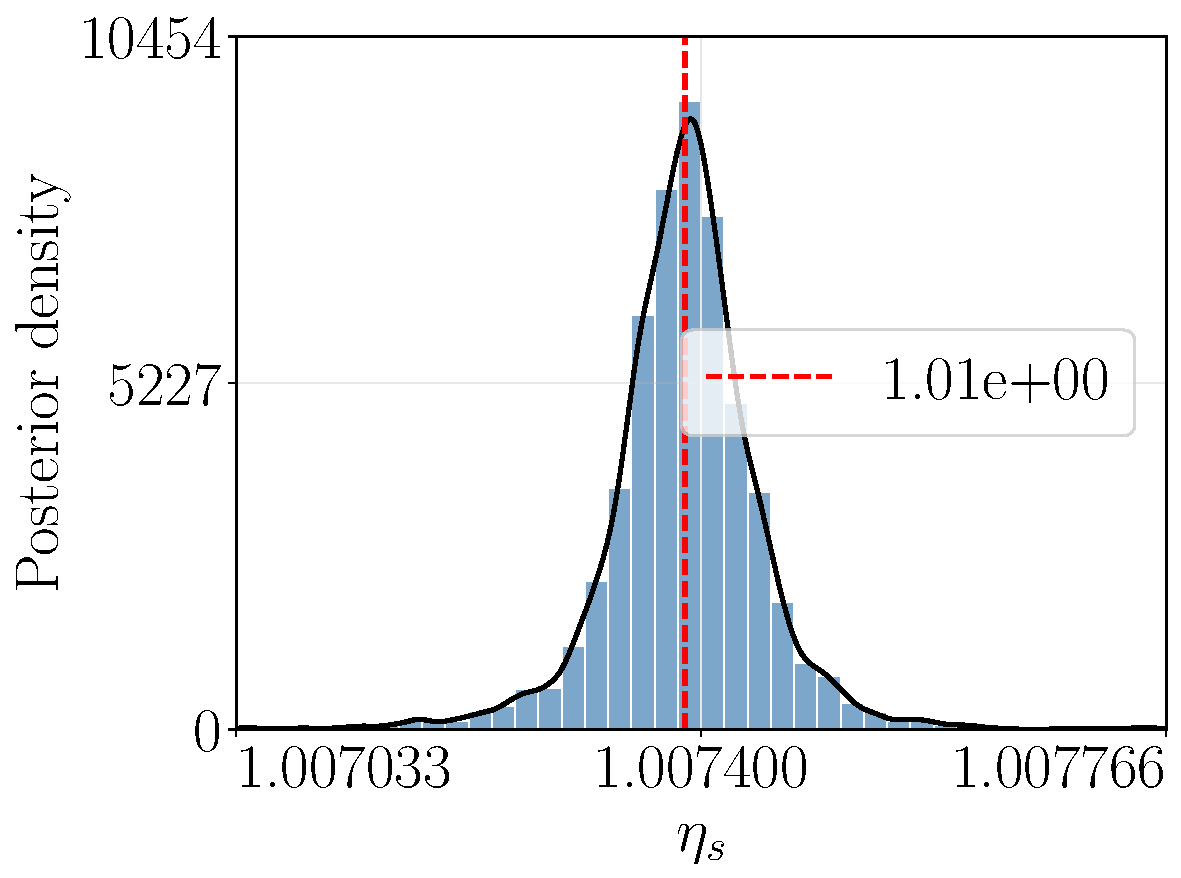
\includegraphics[width=0.33\linewidth]{newtonian/case1/posterior.pdf}
\caption{Marginal posterior distribution of
           $\eta_{\mathrm{s}}$ for the isolated Newtonian particle with
           synthetic noise standard deviation $2\%$ of $u_{\max}$.}
 \label{fig:newtonian_case1_posterior}
\end{figure}

We next examine how the prescribed noise level influences the inference,
considering scales of $0.5\%$, $2\%$, $5\%$, and $10\%$ of $u_{\max}$.
The corresponding noisy trajectories are shown in
Fig.~\ref{fig:sigma_noise_newtonian}, and the posterior summaries in
Table~\ref{tab:noise_newtonian}. The inferred viscosity is robust: even
at $10\%$ noise, $\hat{\eta}_{\mathrm{s}}$ stays within about $1\%$ of
the true value. Increasing the noise mainly broadens the posterior and
raises the inferred experimental-noise standard deviation
$\hat{\sigma}_{\mathrm{exp}}$, both roughly in proportion to the added
noise. This robustness follows from the simplicity of the Newtonian
response: the displacement grows linearly in time, so the inference
reduces to estimating a single slope, and zero-mean scatter about that
line averages out over the trajectory.

\begin{figure}[!ht]
    \centering
    
\includegraphics[width=0.93\linewidth]{newtonian_noise_percent_fixed_axes.pdf}
\caption{Newtonian displacement response with synthetic Gaussian noise
added to the FEM data. The noise is zero-mean with standard deviation
$\sigma_{\mathrm{noise}}$ chosen as a percentage of the maximum displacement
$u_{\max}=\max_t |u(t)|$: $0.5\%$ in the left panel, $2\%$ in the middle
panel, and $5\%$ in the right panel. The red curve denotes the reduced
model prediction, and the black dots denote the FEM simulations.}
  \label{fig:sigma_noise_newtonian}
\end{figure}


\begin{table}[!ht]
\centering
\begin{tabular}{c cc cc}
\toprule
Noise
& $\hat{\eta}_{\subs}$ & $\stdof{\hat{\eta}_{\subs}}$
& $\hat{\sigma}_{\subexp}$ & $\stdof{\hat{\sigma}_{\subexp}}$ \\
\midrule
$0.5\%$
& $1.0$ & $2.36\times 10^{-3}$
& $5.64\times 10^{-2}$ & $1.11\times 10^{-2}$ \\
$2\%$
& $1.0$ & $8.64\times 10^{-3}$
& $2.30\times 10^{-1}$ & $4.40\times 10^{-2}$ \\
$5\%$
& $1.00$ & $2.06\times 10^{-2}$
& $5.71\times 10^{-1}$ & $1.15\times 10^{-1}$ \\
$10\%$
& $1.01$ & $4.18\times 10^{-2}$
& $1.15$ & $2.14\times 10^{-1}$ \\
\bottomrule
\end{tabular}
\caption{Effect of the prescribed noise percentage on inference for the
Newtonian unbounded model. The estimate $\hat{\eta}_{\subs}$ stays within
about one percent of the true value $\eta_{\subs}=1$ at all noise levels,
while the inferred experimental-noise standard deviation $\hat{\sigma}_{\subexp}$
(posterior mean) grows in proportion to the added noise.}
\label{tab:noise_newtonian}
\end{table}

\FloatBarrier

\subsubsection{Viscoelastic fluid}
The Newtonian baseline tests whether a single slope identifies a single
material parameter. We next add memory by considering an Oldroyd-B fluid,
where the same trajectory must identify both viscous and elastic
time-dependent contributions.

\begin{table}[!ht]
\centering
\begin{tabular}{ll}
\toprule
Parameter & Prior \\
\midrule
$\log_{10}\eta_{\mathrm{s}}$      & $\mathcal{U}(\log_{10}(0.01),\,\log_{10}(100))$ \\
$\log_{10}\eta_{\mathrm{p}}$      & $\mathcal{U}(\log_{10}(0.01),\,\log_{10}(100))$ \\
$\log_{10}\lambda$                & $\mathcal{U}(\log_{10}(0.01),\,\log_{10}(100))$ \\
$\log_{10}\delta$                 & $\mathcal{U}(\log_{10}(0.001),\,\log_{10}(100))$ \\
$\ell_{\mathrm{bias}}$            & $\mathcal{U}(0.05,\,0.5)$ \\
$\sigma_{\mathrm{exp}}$           & $\mathcal{E}(\beta_{\mathrm{exp}})$ \\
$\sigma_{\mathrm{bias}}$          & $\mathcal{E}(100)$ \\
\bottomrule
\end{tabular}
\caption{Prior distributions used for the viscoelastic inference cases.}
\label{tab:prior_distributions_viscoelastic}
\end{table}
A particle of radius $a = 1$ is driven by a constant force $F = 8\pi$ at
$\theta = 0^{\circ}$ over $0 \le t \le t_{0} = 0.2$; the force is then
removed and the simulation continues to $t = 0.5$ to capture the full
creep-recovery response. The fluid is Oldroyd-B with true parameters
$\eta_{\mathrm{s}} = 0.5$, $\eta_{\mathrm{p}} = 0.9$, and
$\lambda = 0.1$. The broad log-uniform priors listed in
Table~\ref{tab:prior_distributions_viscoelastic} encode weak prior
knowledge of the rheological parameters.

\begin{figure}[!ht]
    \centering        
\includegraphics[width=\linewidth]{viscoelastic/creep-case1/posterior.pdf}
\caption{Marginal posterior distributions of
$(\eta_{\mathrm{s}},\,\eta_{\mathrm{p}},\,\lambda)$ for the
unbounded-domain creep-recovery case with true parameters
$\eta_{\mathrm{s}} = 0.5$, $\eta_{\mathrm{p}} = 0.9$,
$\lambda = 0.1$. The synthetic noise standard deviation is $2\%$ of the
maximum displacement at $t=t_0=0.2$.}
        \label{viscoelastic:case1-posterior}
\end{figure}

For the posterior in Fig.~\ref{viscoelastic:case1-posterior}, synthetic
zero-mean Gaussian noise is added with standard deviation set to $2\%$ of
the maximum displacement, attained at the end of forcing at $t=t_0=0.2$.
All three parameters are reasonably well constrained, with
the true value of each lying within the posterior uncertainty. A single
creep-recovery trajectory therefore contains enough information to
jointly identify $(\eta_{\mathrm{s}},\,\eta_{\mathrm{p}},\,\lambda)$
within the uncertainty set by the prescribed noise. This is possible
because each parameter governs a distinct feature of the response:
$\eta_{\mathrm{s}}$ controls the initial creep rate, $\lambda$ the
timescale of stress build-up and relaxation, and $\eta_{\mathrm{p}}$
the magnitude of the elastic contribution during recovery.

As in the Newtonian case, we test the sensitivity of the inference to
measurement noise by adding zero-mean Gaussian noise to the FEM
trajectory at $0.5\%$, $2\%$, $5\%$, and $10\%$ of the maximum
displacement $u_{\max}$ (Fig.~\ref{fig:sigma_noise_viscoelastic}), with
the resulting posteriors reported in
Table~\ref{tab:noise_viscoelastic}. The estimates remain accurate up to
about $2\%$ noise, where
$(\eta_{\mathrm{s}},\,\eta_{\mathrm{p}},\,\lambda)$ are still recovered
close to their true values with a small spread. At $5\%$, however, the
inference degrades sharply: $\eta_{\mathrm{p}}$ and $\lambda$ drift well
away from their true values and their standard deviations grow by roughly
two orders of magnitude; by $10\%$, the estimates are no longer
meaningful. This contrast reflects the greater complexity of the
creep-recovery response relative to the Newtonian case.

\begin{figure}[!ht]
    \centering
    
\includegraphics[width=0.95\linewidth]{creep_unbounded_noise_percent_fixed_axes.pdf}
\caption{Viscoelastic displacement response with synthetic Gaussian noise
added to the FEM data. The noise is zero-mean with standard deviation
$\sigma_{\mathrm{noise}}$ chosen as a percentage of the maximum displacement
$u_{\max}=\max_t |u(t)|$: $0.5\%$ in the left panel, $2\%$ in the middle
panel, and $5\%$ in the right panel. The red curve denotes the reduced
model prediction, and the black dots denote the FEM simulations.}
  \label{fig:sigma_noise_viscoelastic}
\end{figure}

\begin{table}[!ht]
\centering
\scriptsize
\resizebox{\textwidth}{!}{%
\begin{tabular}{c cc cc cc cc}
\toprule
Noise
& $\hat{\eta}_{\subs}$ & $\stdof{\hat{\eta}_{\subs}}$
& $\hat{\eta}_{\subp}$ & $\stdof{\hat{\eta}_{\subp}}$
& $\hat{\lambda}$ & $\stdof{\hat{\lambda}}$
& $\hat{\sigma}_{\subexp}$ & $\stdof{\hat{\sigma}_{\subexp}}$ \\
\midrule
$0.5\%$
& $0.549$ & $1.38\times 10^{-2}$
& $0.857$ & $1.42\times 10^{-2}$
& $1.03\times 10^{-1}$ & $3.95\times 10^{-3}$
& $1.08\times 10^{-3}$ & $1.92\times 10^{-4}$ \\
$2\%$
& $0.557$ & $2.67\times 10^{-2}$
& $0.843$ & $2.35\times 10^{-2}$
& $1.03\times 10^{-1}$ & $6.39\times 10^{-3}$
& $3.92\times 10^{-3}$ & $4.08\times 10^{-4}$ \\
$5\%^{\dagger}$
& $0.635$ & $1.55\times 10^{-1}$
& $1.37$ & $1.79$
& $0.747$ & $1.93$
& $9.69\times 10^{-3}$ & $1.17\times 10^{-3}$ \\
$10\%^{\dagger}$
& $1.04$ & $1.24\times 10^{-1}$
& $5.72$ & $2.64$
& $6.14$ & $2.50$
& $1.93\times 10^{-2}$ & $2.37\times 10^{-3}$ \\
\bottomrule
\end{tabular}%
}
\caption{Effect of the prescribed noise percentage on inference for the
unbounded creep-recovery model; $\hat{\sigma}_{\subexp}$ is the posterior
mean of the inferred experimental-noise standard deviation.
At $5\%$ and $10\%$ noise, the posterior standard deviations of $\eta_{\subp}$ and $\lambda$ equal or exceed their means: the polymer
parameters are no longer identified, and the corresponding point estimates
should not be interpreted as material properties.}
\label{tab:noise_viscoelastic}
\end{table}
\FloatBarrier

\subsubsection{Nonlinear viscoelastic}

All preceding viscoelastic experiments were run at moderate Weissenberg
numbers, within the range of validity of the linear surrogate. To locate
where this approximation breaks down,
Fig.~\ref{fig:non_linear_analysis} first scales the forcing relative to
the baseline creep case, with $F=8\pi c$ (so that $c=1$ corresponds to
$F=8\pi$) and the displacement scaled by $c$. Up to approximately $c=32$
($F=256\pi$), the scaled trajectories nearly collapse, indicating an
approximately linear response; for larger forcing, the collapse is lost,
marking the onset of nonlinear viscoelastic effects. We therefore test a
strongly nonlinear case with $F=800\pi$ and $\theta=0^\circ$, for which
$\wi\gg 1$ and the linear creep model is not expected to be
quantitatively accurate.
\begin{figure}[!ht]
    \centering
        \begin{subfigure}[b]{0.32\linewidth}
        
\includegraphics[width=\linewidth]
        {creep_nonlinear.pdf}
    \caption{Force-scaled nonlinear response.}
    \label{fig:non_linear_analysis}
    \end{subfigure}
    \begin{subfigure}[b]{0.33\linewidth}
        \centering
        
\includegraphics[width=\linewidth]
        {viscoelastic/creep-300pi_1e-6/data_vs_noise.pdf}
    \caption{FEM data and reduced model.}
        \label{fig:non-lin-displacement}
    \end{subfigure}
    \begin{subfigure}[b]{0.33\linewidth}
        \centering
        
\includegraphics[width=\linewidth]
        {viscoelastic/creep-300pi_1e-6/posterior_predictive.pdf}
        \caption{Posterior predictive band.}
        \label{fig:non-lin-posterior-predictive}
    \end{subfigure}
    \caption{High-Weissenberg-number creep test at $F = 800\pi$. The reduced linear surrogate underpredicts the nonlinear FEM peak displacement, but a single-trajectory posterior predictive fit can partially mask this structural error by shifting the inferred parameters.}
    \label{fig:nonlinear_single_predictive}
\end{figure}
Figure~\ref{fig:non-lin-displacement} compares the FEM trajectory with
the reduced-order prediction in this high-$\wi$ regime. The surrogate
captures the early-time response reasonably well, where the motion is
governed mainly by viscous resistance. At later times, however, nonlinear
elastic effects become important: the FEM trajectory reaches a larger
peak displacement, and the reduced model underestimates both the peak
displacement and the relaxation amplitude.

\begin{figure}[!ht]
    \centering
    
\includegraphics[width=\linewidth]
    {viscoelastic/creep-300pi_1e-6/posterior.pdf}
\caption{Marginal posterior distributions of
$(\eta_{\mathrm{s}},\,\eta_{\mathrm{p}},\,\lambda)$ for the
nonlinear creep test at $F = 800\pi$ ($\wi \gg 1$). Vertical dashed
lines mark the true parameter values. The estimated $\eta_{\mathrm{p}}$
drifts upward to absorb the unrepresented nonlinear elastic contribution.}
    \label{fig:posterior-nonlin1}
\end{figure}

For a single trajectory, this structural error can be partly hidden by
the posterior predictive fit. The band in
Fig.~\ref{fig:non-lin-posterior-predictive} closely follows the FEM data
because the inferred parameters shift to compensate for the missing
nonlinear physics. This is evident in Fig.~\ref{fig:posterior-nonlin1}:
$\eta_{\mathrm{s}}$ and $\lambda$ remain close to their true values,
while $\eta_{\mathrm{p}}$ shifts upward
($\eta_{\mathrm{p}}^{\mathrm{true}}=0.9$ versus
$\hat{\eta}_{\mathrm{p}}\approx 1.06$), absorbing the nonlinear elastic
contribution that the surrogate cannot represent.

The single-trajectory fit is therefore not a reliable diagnostic of
model adequacy. To expose the model error, we fit several force levels
jointly, so that one biased parameter set cannot compensate for the
missing nonlinearities at all forces simultaneously. We compare a
lower-force set, $F\in\{16\pi,32\pi,64\pi\}$, which stays in the
linear-response regime, with a high-force set,
$F\in\{200\pi,400\pi,800\pi\}$, which enters the high-$\wi$ regime.


\begin{figure}[!ht]
    \centering
    \begin{subfigure}{0.34\linewidth}
        \centering
        
\includegraphics[width=\linewidth]
        {viscoelastic/creep-lin-mix/data_vs_noise.pdf}
        \caption{Linear-regime displacement data.}
        \label{fig:linmix-data-noise}
    \end{subfigure}
    \hspace{0.4cm}
    \begin{subfigure}{0.34\linewidth}
        \centering
        
\includegraphics[width=\linewidth]
        {viscoelastic/creep-lin-mix/posterior_predictive.pdf}
        \caption{Linear-regime posterior predictive.}
        \label{fig:linmix-posterior-predictive}
    \end{subfigure}
    
    % \vspace{0.1cm}

    \begin{subfigure}{0.34\linewidth}
        \centering
        
\includegraphics[width=\linewidth]
        {viscoelastic/creep-non-lin-mix1/data_vs_noise.pdf}
        \caption{High-$\wi$ displacement data.}
        \label{fig:nonlinmix-data-noise}
    \end{subfigure}
    \hspace{0.4cm}
    \begin{subfigure}{0.34\linewidth}
        \centering
        
\includegraphics[width=\linewidth]
        {viscoelastic/creep-non-lin-mix1/posterior_predictive.pdf}
        \caption{High-$\wi$ posterior predictive.}
        \label{fig:nonlinmix-posterior-predictive}
    \end{subfigure}
    \caption{Joint posterior predictive checks for mixed creep-recovery
    data. The left panels show the displacement curves, and the right
    panels show the posterior predictive bands. The lower-force set
    $F \in \{16\pi,\,32\pi,\,64\pi\}$ is described well by the surrogate,
    whereas the high-force set
    $F \in \{200\pi,\,400\pi,\,800\pi\}$ shows systematic deviations near
    peak displacement and during recovery, revealing the limit of the
    linear viscoelastic surrogate.}
    \label{fig:predictive_posterior-nonlin1}
\end{figure}

Figure~\ref{fig:predictive_posterior-nonlin1} shows the resulting
posterior predictive checks. For the lower-force set, the surrogate
describes all three trajectories well. For the high-force set,
systematic discrepancies grow with $F$, especially near the peak
displacement and during recovery. The joint fit therefore reveals that
the discrepancy is not merely a poor point estimate but evidence of
unrepresented nonlinear physics in the forward model.

\FloatBarrier

\subsection{Wall effects}
\subsubsection{Newtonian fluid}
We now introduce a wall and first consider wall-parallel motion. In the
wall-corrected Stokes relation, the resistance depends on the product
$\eta_{\mathrm{s}} f_{\parallel}(\delta/a)$, so increasing the viscosity
or decreasing the wall distance reduces the particle mobility in the same
way. From a single wall-parallel trajectory, these two effects cannot be
separated: many pairs $(\eta_{\mathrm{s}},\delta)$ produce the same
displacement slope.

For this parallel-motion case, the identifiable quantity is the effective
mobility parameter
\begin{equation}
\kappa = \dfrac{1}{f_{\parallel}(\delta/a)\,\eta_{\mathrm{s}}},
\label{eq:kappa}
\end{equation}
which captures the combined effect of viscosity and wall-induced parallel
resistance. For trajectories generated with $F = 12\pi$ at
$\theta = 0^{\circ}$ and $\delta/a = 0.1$, the reference effective
mobility is $\kappa = 0.443$. As shown in
Fig.~\ref{fig:newtonian:case2-posterior}, the posterior concentrates
around this value, confirming that $\kappa$ is well identified.

\begin{figure}[!ht]
\centering
\begin{subfigure}[b]{0.34\linewidth}
  \centering
  
\includegraphics[width=\linewidth]{newtonian/case2-kappa/posterior.pdf}
  \caption{$\delta/a = 0.1$.}
  \label{fig:newtonian:case2-kappa-01}
\end{subfigure}

\caption{Posterior distribution of the effective mobility $\kappa$ in the bounded domain at $\delta/a = 0.1$.}
\label{fig:newtonian:case2-posterior}
\end{figure}

The single-direction experiment thus fixes only the parallel mobility
$\kappa$, providing a single observable, the slope $\dot{x}$, and cannot
separate $\eta_{\mathrm{s}}$ from $\delta$. Oblique forcing breaks this
degeneracy by producing both wall-parallel and wall-perpendicular motion:
any angle $\theta \in (0^{\circ},90^{\circ})$ yields two independent
slopes,
\begin{equation}
\dot{x}
=
\frac{F\cos\theta}
{6\pi\,a\,\eta_{\mathrm{s}}\,f_{\parallel}(\delta/a)},
\qquad
\dot{y}
=
\frac{F\sin\theta}
{6\pi\,a\,\eta_{\mathrm{s}}\,f_{\perp}(\delta/a)},
\label{eq:slopes_oblique}
\end{equation}
whose ratio
\begin{equation}
\frac{\dot{y}}{\dot{x}}
=
\tan\theta\,
\frac{f_{\parallel}(\delta/a)}{f_{\perp}(\delta/a)}
\label{eq:slope_ratio}
\end{equation}
depends only on $\delta/a$, since the viscosity cancels. The two
resistance factors diverge at different rates as $\delta/a \to 0$
($f_{\parallel}$ logarithmically, $f_{\perp}$ algebraically), so their
ratio $f_{\parallel}/f_{\perp}$ varies strongly over the near-wall range
considered. The slope ratio therefore provides direct information about
$\delta$, after which either component of Eq.~\eqref{eq:slopes_oblique}
fixes $\eta_{\mathrm{s}}$. The choice $\theta = 45^{\circ}$ used here
balances the sensitivities of
$\dot{x}$ and $\dot{y}$ and is adopted for definiteness; the argument
applies equally to any $\theta \in (0^{\circ}, 90^{\circ})$.

We now examine whether $\eta_{\mathrm{s}}$ and $\delta$ can be jointly
identified from a bounded-domain trajectory generated with oblique
forcing, $F=12\pi$ at $\theta=45^\circ$, $\delta/a=0.1$, and synthetic
noise standard deviation $2\%$ of $u_{\max}$.
Figure~\ref{newtonian:case3-corner} shows the
marginal posteriors and the correlation between $\eta_{\mathrm{s}}$ and
$\delta$. The posterior uncertainty contains the true value of each
parameter, the posterior means lie close to them, and the off-diagonal
panel shows a strong positive correlation between the two.

The preceding results use the wall-corrected forward model. To isolate
the effect of model error, Fig.~\ref{fig:newtonian_model_error} instead
fits the unbounded Newtonian model to bounded-domain FEM data at
$\delta/a=0.01$. For wall-parallel forcing ($\theta=0^\circ$), the
posterior predictive still follows the data closely, but only by
inferring biased parameters that compensate for the omitted wall drag. At
$\theta=45^\circ$ this compensation becomes less effective and the band
widens; for wall-normal forcing ($\theta=90^\circ$), where the wall
correction is strongest, it widens further and the mismatch becomes most
apparent. The posterior predictive thus reveals the growing structural
error as the motion becomes more wall-normal.

\begin{figure}[!ht]
    \centering

\includegraphics[width=0.45\linewidth]
    {newtonian/case3-eta_delta-0.1/corner.pdf}
\caption{Marginal posterior distributions and correlation between
$\eta_{\mathrm{s}}$ and $\delta$ for the bounded-domain Newtonian case
at $\delta/a = 0.1$. Diagonal panels show the 1D marginal posteriors; dashed vertical lines mark the 95\% credible interval, and the red
curves show the prior densities in the plotted coordinates. The off-diagonal panel
shows the correlation between the two parameters, with contours
enclosing the 68\% and 95\% credible regions.}
    \label{newtonian:case3-corner}
\end{figure}

\begin{figure}[!ht]
\centering
\begin{subfigure}[b]{0.32\linewidth}
  \centering
  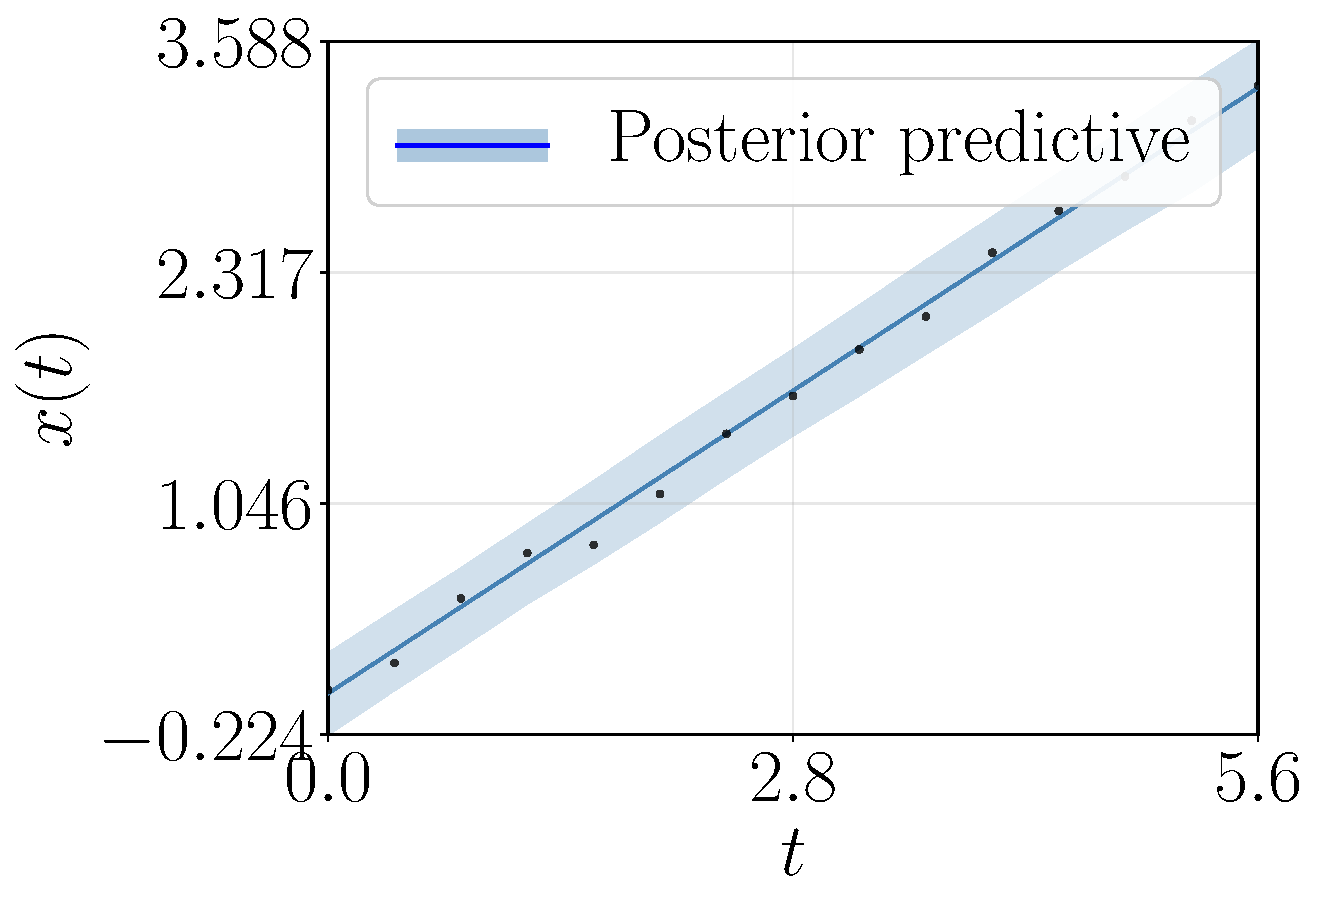
\includegraphics[width=\linewidth]{newtonian/model_error/posterior_predictive_0.01_0.pdf}
  \caption{$\delta/a = 0.01, \theta = 0^{\circ}$.}
  \label{fig:newtonian:case2-kappa-01-b}
\end{subfigure}
\begin{subfigure}[b]{0.32\linewidth}
  \centering
  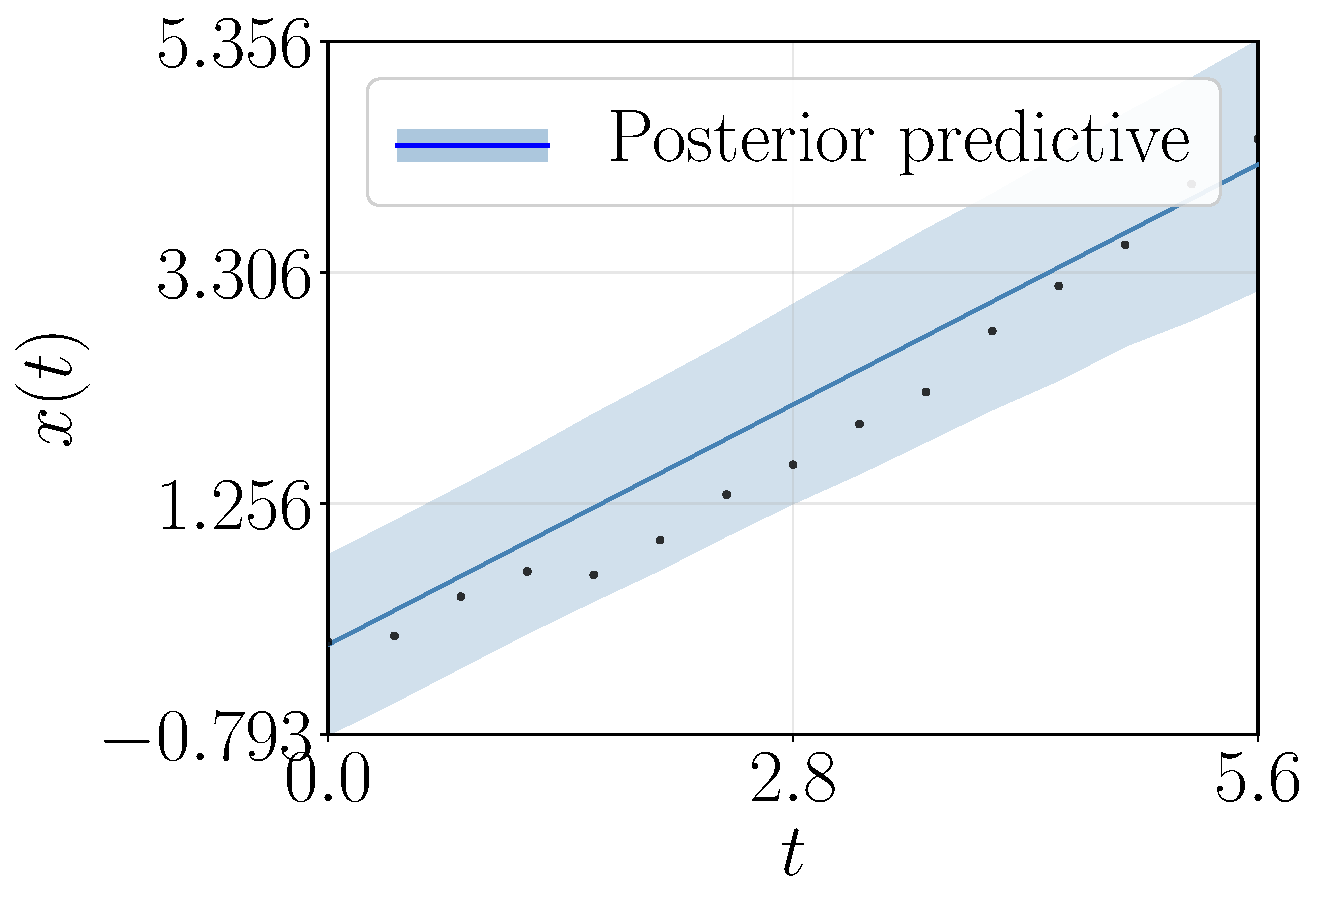
\includegraphics[width=\linewidth]{newtonian/model_error/posterior_predictive_0.01_45.pdf}
  \caption{$\delta/a = 0.01, \theta = 45^{\circ}$.}

\end{subfigure}
\begin{subfigure}[b]{0.32\linewidth}
  \centering
  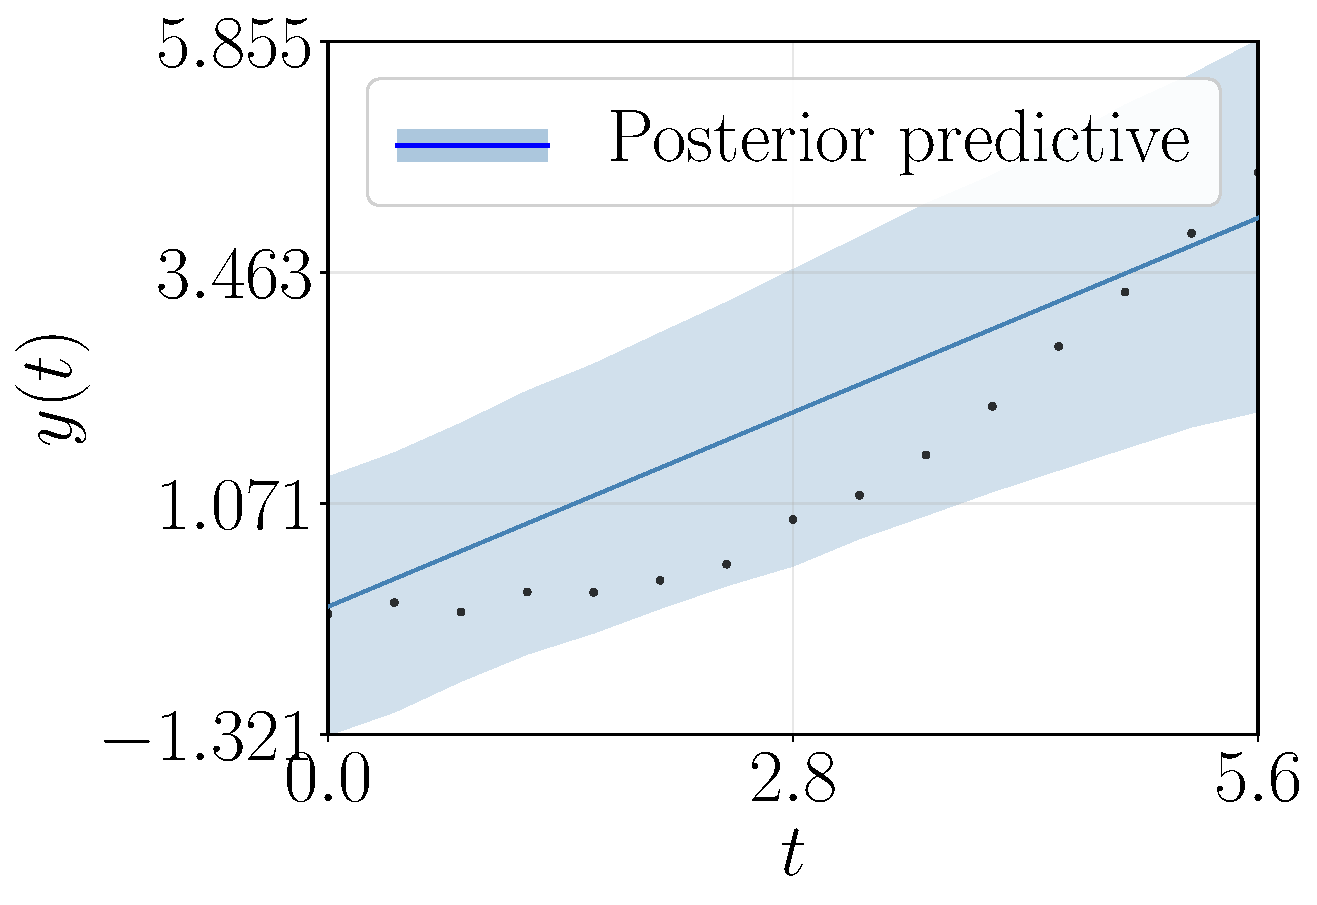
\includegraphics[width=\linewidth]{newtonian/model_error/posterior_predictive_0.01_90.pdf}
  \caption{$\delta/a = 0.01, \theta = 90^{\circ}$.}
  \label{fig:newtonian:case2-kappa-001b}
\end{subfigure}
\caption{Posterior predictive bands obtained when the unbounded
Newtonian model is fit to bounded-domain FEM data at
$\delta/a = 0.01$. The mismatch increases from wall-parallel forcing to
wall-normal forcing, consistent with the increasing importance of the
omitted wall correction.}
\label{fig:newtonian_model_error}
\end{figure}

Table~\ref{delta-newtonian} reports posterior means and standard
deviations for $\eta_{\mathrm{s}}$ and $\delta$ at three true gap
distances, with $\eta_{\mathrm{s}}=1$ and baseline noise. In every case
the posterior means are close to the true values and the posterior
uncertainty contains the truth, including at the smallest gap
$\delta=0.001$, where wall effects are strongest.

\begin{table}[!ht]
\centering
\begin{tabular}{c l cc}
\toprule
True $\delta$ & Parameter & Mean & Std \\
\midrule
\multirow{2}{*}{0.001}
 & $\eta_{\mathrm{s}}$ & 1.004 & $1.7\times 10^{-3}$ \\
 & $\delta$            & 0.001 & $1.9\times 10^{-5}$ \\
\midrule
\multirow{2}{*}{0.01}
 & $\eta_{\mathrm{s}}$ & 0.9987 & $6.8\times 10^{-4}$ \\
 & $\delta$            & 0.0097 & $7.2\times 10^{-5}$ \\
\midrule
\multirow{2}{*}{0.1}
 & $\eta_{\mathrm{s}}$ & 0.9984 & $6.8\times 10^{-4}$ \\
 & $\delta$            & 0.095  & $7.9\times 10^{-4}$ \\
\bottomrule
\end{tabular}
\caption{Posterior mean and standard deviation for $\eta_{\mathrm{s}}$
         and $\delta$ at three true wall distances, with fixed
         $\eta_{\mathrm{s}} = 1$ at baseline noise.}
\label{delta-newtonian}
\end{table}

\FloatBarrier

\subsubsection{Viscoelastic fluid}

Having analyzed isolated creep-recovery trajectories, we now add the wall
separation as a fourth unknown. This bounded viscoelastic problem
combines the two identifiability mechanisms seen above: the transient
shape separates $(\eta_{\mathrm{s}},\,\eta_{\mathrm{p}},\,\lambda)$, while
the oblique trajectory separates the wall-parallel and wall-normal
mobilities needed to infer $\delta$. We therefore use $\theta=45^{\circ}$,
so that both mobility components are excited in the same experiment.

For the representative case $\delta/a = 0.1$,
Fig.~\ref{creep:case2-corner} shows the marginal and joint posteriors of
$(\eta_{\mathrm{s}},\,\eta_{\mathrm{p}},\,\lambda,\,\delta)$. The diagonal
panels show unimodal marginals concentrated well inside the broad prior
ranges, indicating that the trajectory is informative about all four
unknowns. The off-diagonal panels reveal a clear correlation between the
wall separation $\delta$ and the two viscosities $\eta_{\mathrm{s}}$ and
$\eta_{\mathrm{p}}$, since both a smaller gap and larger viscosities
reduce mobility. By contrast, $\lambda$ remains nearly uncorrelated with
$\delta$, indicating that the inferred relaxation time is largely
unaffected by wall effects.

    \begin{figure}[!ht]
        \centering
    
\includegraphics[width=0.8\linewidth]
        {viscoelastic/creep-delta-0.1/corner.pdf}
        \caption{Marginal and joint posterior distributions of
$(\eta_{\mathrm{s}},\,\eta_{\mathrm{p}},\,\lambda,\,\delta)$ for the
bounded-domain creep-recovery case at $\delta/a = 0.1$. Diagonal panels
show the 1D marginal posteriors; dashed vertical lines mark the 95\%
credible interval. Off-diagonal panels show the 2D joint posteriors,
with contours enclosing the 68\% and 95\% credible regions.}
        \label{creep:case2-corner}
\end{figure}


\begin{table}[!ht]
\centering
\begin{tabular}{c l c c c}
\toprule
True $\delta$ & Parameter & True value & Mean & Std \\
\midrule
\multirow{4}{*}{0.005}
 & $\eta_{\mathrm{s}}$      & 0.50 & 0.46  & $1.5\times 10^{-2}$ \\
 & $\eta_{\mathrm{p}}$      & 0.90 & 0.92  & $3.1\times 10^{-2}$ \\
 & $\lambda$                & 0.10 & 0.095 & $1.4\times 10^{-3}$ \\
 & $\delta$                 & 0.005& 0.0049& $1.1\times 10^{-3}$ \\
\midrule
\multirow{4}{*}{0.01}
 & $\eta_{\mathrm{s}}$      & 0.50 & 0.46  & $7.1\times 10^{-3}$ \\
 & $\eta_{\mathrm{p}}$      & 0.90 & 0.92  & $1.2\times 10^{-2}$ \\
 & $\lambda$                & 0.10 & 0.098 & $1.1\times 10^{-3}$ \\
 & $\delta$                 & 0.010& 0.0097& $7.3\times 10^{-4}$ \\
\midrule
\multirow{4}{*}{0.1}
 & $\eta_{\mathrm{s}}$      & 0.50 & 0.47  & $5.2\times 10^{-3}$ \\
 & $\eta_{\mathrm{p}}$      & 0.90 & 0.96  & $8.8\times 10^{-3}$ \\
 & $\lambda$                & 0.10 & 0.094 & $1.3\times 10^{-3}$ \\
 & $\delta$                 & 0.100& 0.100 & $2.4\times 10^{-3}$ \\
\bottomrule
\end{tabular}
\caption{Posterior mean and standard deviation at three true gap
         distances, with true parameters $\eta_{\mathrm{s}} = 0.5$,
         $\eta_{\mathrm{p}} = 0.9$, and $\lambda = 0.1$.}
\label{tab:creep-delta}
\end{table}

Table~\ref{tab:creep-delta} reports the posterior means and standard
deviations for
$(\eta_{\mathrm{s}},\,\eta_{\mathrm{p}},\,\lambda,\,\delta)$ at three
true wall distances, $\delta \in \{0.005, 0.01, 0.1\}$. The posterior
means stay close to the true values across the tested gaps, but a small
systematic bias is visible: the solvent viscosity is underestimated by
about $6$ to $8\%$, and the polymer viscosity is overestimated by up to
about $7\%$. The relaxation time and wall separation are recovered more
tightly. This small offset is consistent with the steady-drag closure
$C=6\pi a^{2}$ introduced in Section~\ref{sec:ve_unbounded}: matching
the polymeric drag at steady state leaves the transient creep amplitude
only approximately represented, so the inference compensates by trading
a slightly lower $\eta_{\mathrm{s}}$ against a slightly higher
$\eta_{\mathrm{p}}$. The discrepancy is small and correlated in time, so
the Gaussian-process bias term absorbs the residual without compromising
the identifiability of the four parameters.

\FloatBarrier

\subsection{Particle-particle interactions}
\label{sec:pp_results}

The wall corrections of the previous sections isolate a single probe from
one boundary. In a suspension, however, the probe also feels its
neighbors. We model this second interaction through the periodic Hasimoto
correction of Section~\ref{sec:hasimoto} and test it in two settings: a
homogeneous material, where the modulus does not vary in space and the
correction can be verified directly, and a heterogeneous material, where
the local modulus varies in space and single-particle probing is compared
against a bulk measurement.

\subsubsection{Homogeneous material}
\label{sec:pp_homogeneous}

In the homogeneous material, the true modulus is prescribed as
$G_{\mathrm{true}} = 9$. When the Hasimoto correction is omitted, the
finite size of the periodic box biases the inferred modulus.
Table~\ref{tab:hasimoto_homogeneous} shows that $G$ is strongly
overestimated for small domains: the raw inference returns
$G_{\mathrm{inferred}} = 19.71$ at $L = 5$, more than twice the true
value. The error falls steadily as the box grows, reaching about $7\%$ at
$L = 60$. This residual offset decays only algebraically with box size,
because the periodic images interact through a slowly decaying Stokes
field; this is precisely the contribution that the Hasimoto factor
removes. Applying the correction is therefore what makes single-particle
inference reliable, and we carry the same correction into the spatially
varying material considered next.

\begin{table}[!ht]
\centering
\begin{tabular}{cccc}
\toprule
$L$ & $G_{\mathrm{inferred}}$ & $\stdof{G_{\mathrm{inferred}}}$ & Error (\%) \\
\midrule
5  & 19.71 & 0.770 & 119 \\
10 & 12.71 & 0.480 & 41.2 \\
20 & 10.67 & 0.407 & 18.6 \\
30 & 10.09 & 0.380 & 12.1 \\
40 & 9.83  & 0.369 & 9.2 \\
60 & 9.63  & 0.390 & 7.0 \\
\bottomrule
\end{tabular}
\caption{Effect of domain size on the inferred modulus in a homogeneous
material with $G_{\mathrm{true}} = 9$ when the Hasimoto correction is
\emph{not} applied. The error is the relative deviation of
$G_{\mathrm{inferred}}$ from $G_{\mathrm{true}}$.}
\label{tab:hasimoto_homogeneous}
\end{table}

\FloatBarrier

\subsubsection{Heterogeneous material}
\label{sec:heterogeneous_inference}

We now turn to a material in which the modulus varies in space,
$G = G(\vec{x})$, while the relaxation time $\lambda$ is held fixed and
uniform. The construction of the heterogeneous microstructure in the
full-order model is described in Section~\ref{sec:blobs}. Here the field is
represented as a uniform background $G_0$ plus a superposition of
$N_b = 20$ Gaussian blobs,
\begin{equation}
G(\vec{x}) = G_0 + \sum_{i=1}^{N_b} A_i \,
\exp\!\left(-\frac{\lVert \vec{x} - \vec{c}_i \rVert_2^2}
{2\,w_i^2}\right),
\label{eq:G_field}
\end{equation}
where each blob width $w_i$ equals its radius $R_i$. The radius and
amplitude of each blob are drawn independently from
$R_i \in \{0.5, 1.0, 1.5, 2.0\}$ and $A_i \in \{2, 5, 10, 20\}$, and the
$N_b$ centers $\vec{c}_i$ are placed by Latin-hypercube sampling for even
spatial coverage. With $G_0 = 9.0 = \eta_{\mathrm{p}}/\lambda$, the
background reproduces the homogeneous reference case, and
$L_x = L_y = L_z = 10$. Because the blob widths satisfy $w_i \ll L$, the
periodic images of each Gaussian contribute negligibly at the box center,
so $G_0$ is recovered as the background modulus away from the peaks.
Figure~\ref{fig:g_heterogeneous_medium}(a) shows the resulting
isosurfaces of $G$, and panel (b) shows planar slices at
$z = -2.5,\, 0,\, +2.5$: smooth, well-separated peaks
($G \sim 30\text{--}34$) sit on a lower background
($G \sim 10\text{--}13$).

\begin{figure}[!ht]
    \centering
    \begin{subfigure}{0.33\linewidth}
        \centering
        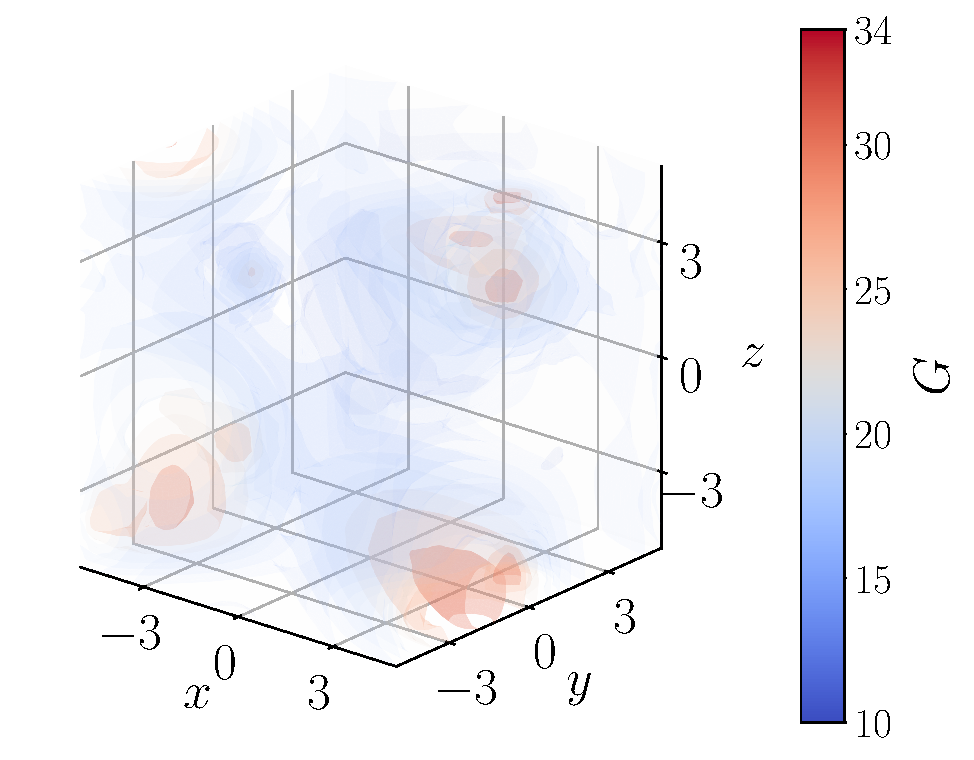
\includegraphics[width=\linewidth]{particle-particle/G_isosurface.pdf}
        \caption{Three-dimensional isosurfaces of the heterogeneous
                 modulus $G$.}
        \label{fig:G_field}
    \end{subfigure}
    \begin{subfigure}{\linewidth}
        \centering
        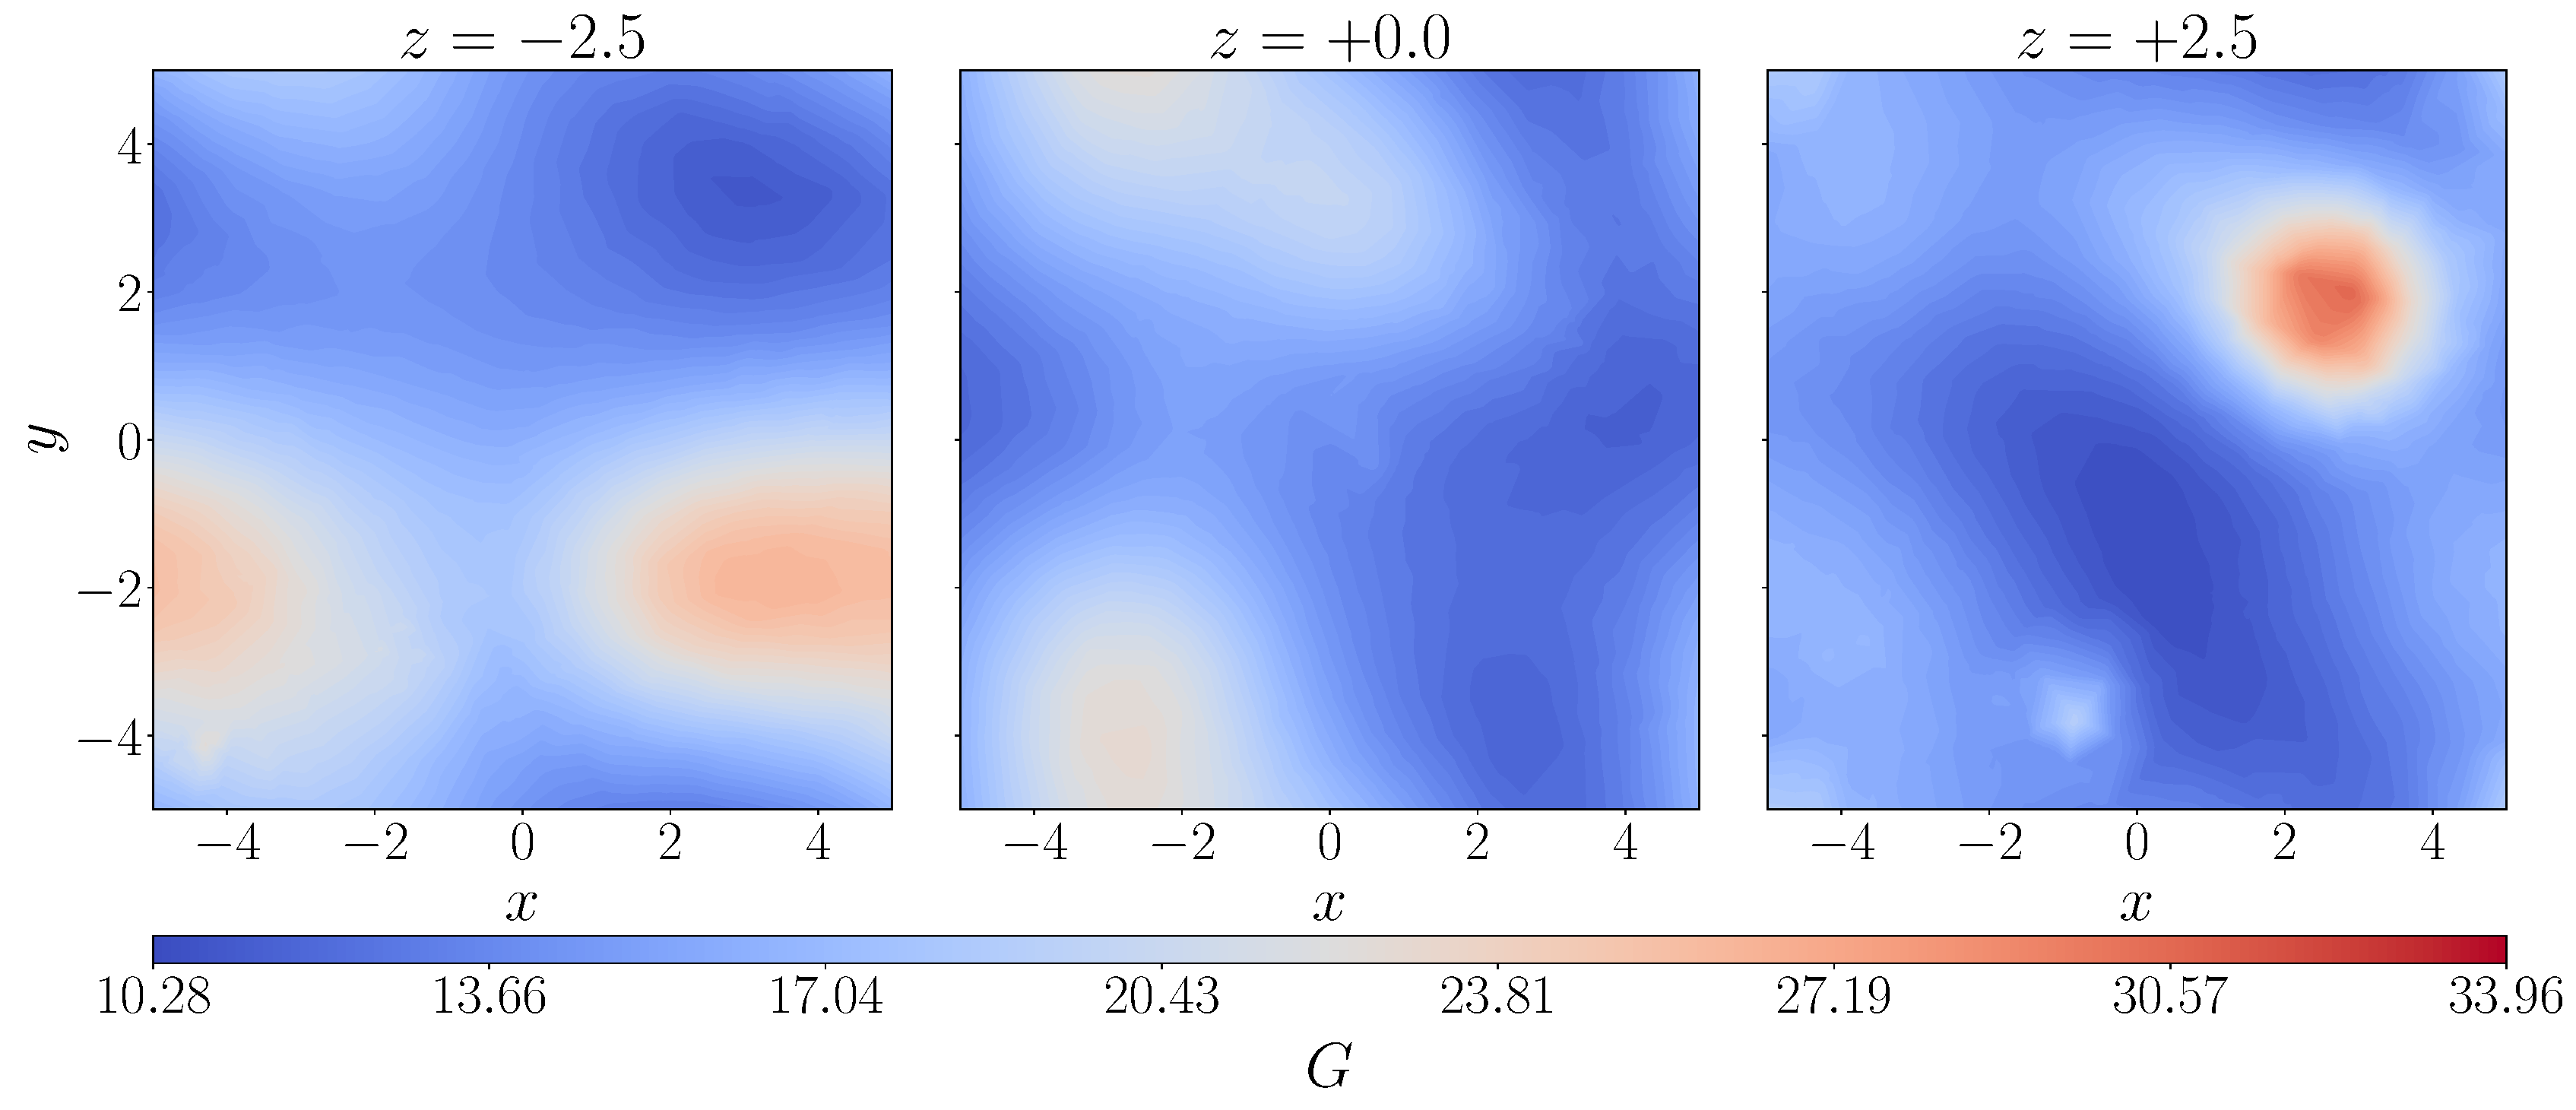
\includegraphics[width=0.7\linewidth]{particle-particle/G_slices_combined.pdf}
        \caption{Planar slices of $G$ at $z = -2.5$, $z = 0$, and
                 $z = 2.5$.}
        \label{fig:g_slices}
    \end{subfigure}
    \caption{Visualization of the heterogeneous modulus field $G$. The
             isosurfaces highlight the three-dimensional heterogeneity,
             while the slices show the spatial variation through the
             domain.}
    \label{fig:g_heterogeneous_medium}
\end{figure}

The central question in a heterogeneous material is what a single moving
probe actually measures: the pointwise modulus at its location, a local
spatial average over the region it disturbs, or the bulk modulus of the
material. Because the probe stress samples the field over a region set by
the particle size, we expect it to report a local, weighted effective
modulus rather than the pointwise value $G(\vec{x}_{\mathrm{p}})$. We
address this by comparing three quantities: the distribution of local
estimates $G_{\mathrm{loc}}$ obtained from many probe configurations,
their mean $\bar{G}_{\mathrm{loc}}$, and an independent bulk modulus
$G_{\mathrm{bulk}}$ from macroscopic shear.

The probe interacts with its own periodic images exactly as in the
homogeneous case, so the same finite-size correction of
Section~\ref{sec:hasimoto} removes the periodic-box artifact before the
particle response is converted into an apparent modulus. Each local
estimate is obtained from the full posterior, with the modulus
$G=\eta_{\mathrm{p}}/\lambda$ evaluated from the posterior samples of
$\eta_{\mathrm{p}}$ and $\lambda$ rather than from their means alone, so
that the reported $G_{\mathrm{loc}}$ carries the inference uncertainty.
To sample the field without regenerating the particle mesh, the particle
is held fixed at the box center and the entire periodic field is
translated rigidly by a random offset $\vec{s} = (s_x, s_y, s_z)$, with
each component drawn uniformly on $[0, L)$ and wrapped periodically. This
is equivalent to evaluating $G(\vec{x} + \vec{s})$ at the fixed particle
location. A new offset is drawn for each of $N_{\mathrm{run}} = 40$
independent runs, giving $40$ independent, Hasimoto-corrected local
estimates $G_{\mathrm{loc}}^{(k)}$ of the shear modulus. Their histogram
(Fig.~\ref{fig:G_histogram}) has mean
\begin{equation}
\bar{G}_{\mathrm{loc}}
= \frac{1}{40} \sum_{k=1}^{40} G_{\mathrm{loc}}^{(k)}
= 17.44.
\label{eq:G_loc_mean}
\end{equation}

\begin{figure}[!ht]
    \centering
    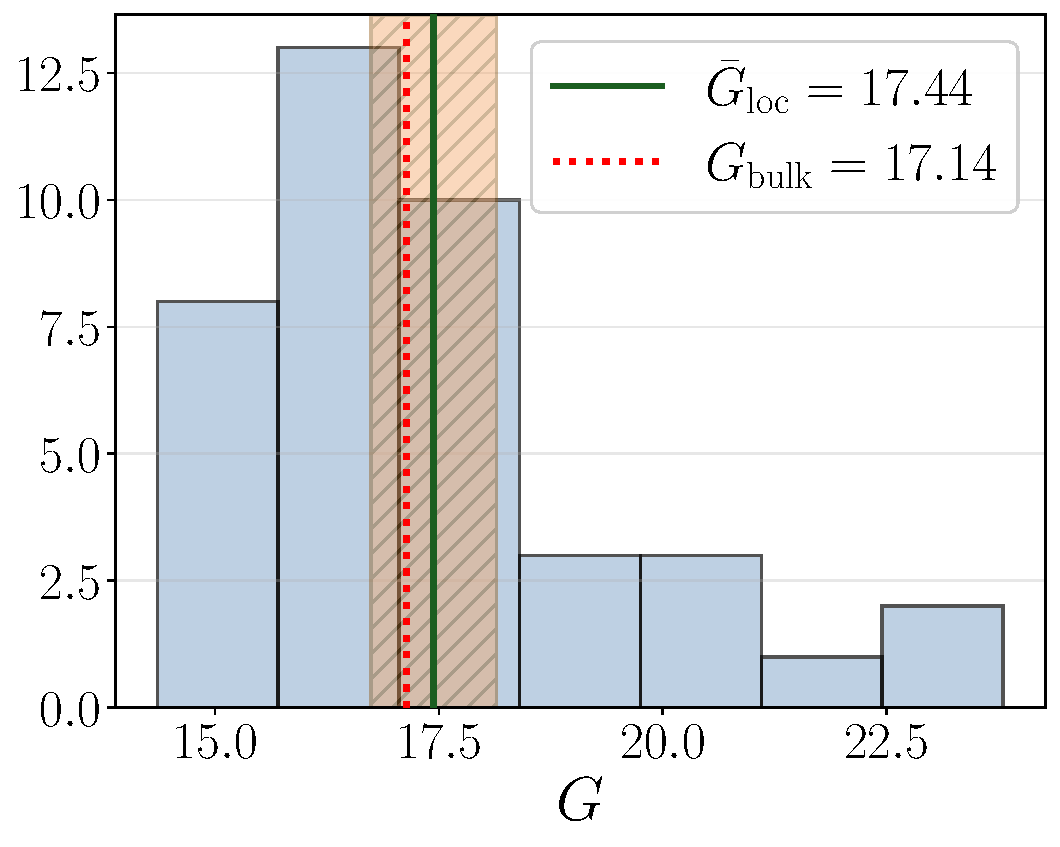
\includegraphics[width=0.29\linewidth]{particle-particle/values_histogram_40.pdf}
    \caption{Histogram of the $40$ Hasimoto-corrected local estimates
             $G_{\mathrm{loc}}^{(k)}$ (mean
             $\bar{G}_{\mathrm{loc}} = 17.44$), shown with the $95\%$
             confidence interval and the bulk reference
             $G_{\mathrm{bulk}} = 17.14$.}
    \label{fig:G_histogram}
\end{figure}

As a reference, the same field is probed in bulk, with no particle
present. A homogeneous simple shear is imposed through Lees--Edwards
periodic boundary conditions: a velocity jump
$\Delta u = u_x(\mathrm{top}) - u_x(\mathrm{bottom})$ across the periodic
$y$-faces sets a macroscopic shear rate $\dot\gamma = \Delta u / L_y$,
and the volume-averaged shear stress $\langle \sigma_{xy} \rangle$ is
tracked in time. Starting from a stress-free state, the first strain
increment $\Delta\gamma = \dot\gamma\,\Delta t$ probes the purely
elastic, pre-relaxation response of the material, so the bulk modulus is
the secant slope of stress over strain at this first step,
\begin{equation}
G_{\mathrm{bulk}}
= \frac{\Delta \langle \sigma_{xy} \rangle}{\Delta\gamma}
= 17.14.
\label{eq:G_bulk_secant}
\end{equation}

The $95\%$ confidence interval of $\bar{G}_{\mathrm{loc}}$ brackets
$G_{\mathrm{bulk}}$, so the two measurements are statistically consistent
in the mean. What each reveals, however, is different.
$G_{\mathrm{bulk}}$ is a single number, blind by construction to the
spatial structure of Fig.~\ref{fig:g_heterogeneous_medium}: it would be
unchanged if the material were exactly uniform at $17.14$. The
particle-resolved estimates instead recover the full distribution, whose
spread is direct evidence of the underlying heterogeneity. This answers
the question posed above: the single-particle probe measures neither the
pointwise modulus nor the bulk value, but a local effective modulus. Its
scatter reflects the spatial variation of the field. Bulk rheology alone
therefore gives an incomplete picture of the material, whereas
Hasimoto-corrected single-particle probing resolves both the local
modulus and its distribution.

\FloatBarrier

\section{Conclusions}
\label{sec:conclusions}

The central theme of this work is that active microrheology becomes
quantitatively reliable only when the systematic biases introduced by the
measurement environment are corrected and the residual uncertainty is
propagated into the inferred parameters. Left uncorrected, wall drag,
finite periodic-domain effects, particle-particle interactions,
heterogeneous sampling, and viscoelastic model inadequacy at high
Weissenberg number each distort the inferred rheology. We have
investigated whether the transient creep-recovery trajectory of
a force-controlled sphere translating near a rigid wall can be used to
infer, in a single experiment, the solvent viscosity, polymer viscosity,
and relaxation time of a viscoelastic fluid, together with the
particle-to-wall separation, once these corrections are in place. Within
the moderate-$\wi$ regime where the
linearized viscoelastic surrogate remains valid, the answer is
affirmative. The Bayesian formulation further provides principled
diagnostics, through posterior predictive checks and an explicit
Gaussian-process bias model, to identify when the experiment has entered
a regime where the surrogate no longer adequately describes the
observations.

The main findings are as follows. (i) For Newtonian fluids, both the
viscosity $\eta_{\mathrm{s}}$ and the particle-to-wall separation
$\delta$ are identifiable from two-directional force-controlled
trajectories, while the unbounded Newtonian baseline remains robust even
when synthetic noise reaches $10\%$ of the maximum displacement. In bounded
geometries, the naturally identifiable quantity from a single-direction
trajectory is the combined mobility parameter
$\kappa = [f_{\parallel}(\delta/a)\,\eta_{\mathrm{s}}]^{-1}$;
separating $\eta_{\mathrm{s}}$ and $\delta$ requires two-directional
forcing data or an independent geometric measurement. (ii) For linear
viscoelastic fluids, creep-recovery trajectories contain sufficient
information to jointly identify the three constitutive parameters and,
under oblique forcing, the wall separation. The joint posterior reflects
the Oldroyd-B coupling structure, including the correlations between
wall separation and viscosity, and between $\eta_{\mathrm{p}}$ and
$\lambda$. (iii) At large Weissenberg number ($\wi \gg 1$), a single
trajectory can be fit by biased effective parameters, but joint
posterior predictive checks across multiple force levels expose the
structural mismatch. (iv) For periodic particle-particle interactions,
the Hasimoto correction removes the dominant finite-domain mobility
artifact, enabling single-particle estimates to recover the distribution
of a heterogeneous modulus field rather than only its bulk average.

Practical guidance on the applicable regime can be summarized as a
validity map in the control parameters $\wi$, the dimensionless gap
$\delta/a$, and the dimensionless box size $L/a$. For
$\wi \ll 1$, moderate gaps, and sufficiently large $L/a$, the linear
surrogate can be applied directly, and the
posterior uncertainty provides a meaningful measure of parameter
identifiability. As $\wi$ approaches or exceeds unity, or as the gap
becomes very small, the bias term and
posterior predictive checks become essential diagnostics rather than
optional uncertainty estimates. For $\wi \gg 1$, posterior predictive
failure should be interpreted as a cue to adopt a nonlinear forward
model or an accurate emulator, and parameters inferred with the
linear-regime surrogate should be treated as effective qualitative
descriptors only. At small $L/a$ the Hasimoto correction is required to
remove the finite-domain bias before any modulus is reported.

Future directions include (i) multi-mode relaxation spectra, replacing
the single-mode Maxwell surrogate with a discrete sum of relaxation
modes; (ii) nonlinear constitutive inference (\eg Giesekus model),
enabled by surrogate models or emulators that reduce the cost of
repeated forward evaluations within MCMC; and (iii) application to
experimental particle-tracking data, where careful treatment of model
bias and instrumental systematics is essential.

\appendix

\section{Mesh and domain-size convergence studies}
\label{sec:mesh_conv}

Two sources of discretization error are assessed for both Newtonian and
viscoelastic settings: (i) the spatial element size (mesh convergence)
and (ii) the size of the truncated computational box (domain-size
convergence). Both studies are reported for the three-dimensional (3D)
bounded geometry and the axisymmetric unbounded geometry.

The mesh hierarchies and domain-size levels are summarized in
Tables~\ref{tab:3d-domain} and~\ref{tab:axi-domain}. Here, $h_{\mathrm{particle}}$ denotes the characteristic element size near
the particle surface and $h_{\mathrm{far}}$ denotes the characteristic size in
the far field.

For the 3D bounded geometry, the convergence of the Newtonian and
viscoelastic solutions is shown in
Figs.~\ref{fig:stokes_conv_3d} and~\ref{fig:creep_3d}, respectively.
For the axisymmetric unbounded geometry, the corresponding results are
given in Figs.~\ref{fig:stokes_conv_axi} and~\ref{fig:creep_axi}.

The particle displacement is found to converge at mesh M3 on domain D2
in the 3D geometry ($\delta/a = 0.1$) and at mesh M2 on domain D2 in
the axisymmetric geometry for both Newtonian and viscoelastic cases.
These discretizations are adopted as the reference configuration for all
subsequent simulations.

\begin{table}[!ht]
  \centering
  \begin{subtable}[t]{0.58\textwidth}
    \centering
    \begin{tabular}{lcccc}
      \toprule
      Mesh & $h_{\mathrm{particle}}$ & $h_{\mathrm{far}}$ & nodes  & elements \\
      \midrule
      M1 & 0.8 & 48 &  1\,242 &     540 \\
      M2 & 0.4 & 24 &  3\,555 &   1\,827 \\
      M3 & 0.2 & 12 & 13\,918 &   8\,380 \\
      M4 & 0.1 &  6 & 85\,766 &  57\,644 \\
      \bottomrule
    \end{tabular}
    \caption{3D mesh hierarchy on the reference domain D2.}
  \end{subtable}\hfill
  \begin{subtable}[t]{0.38\textwidth}
    \centering
    \begin{tabular}{cccc}
      \toprule
      Domain & $L$ & $W$ & $H$ \\
      \midrule
      D1 &  50 &  50 &  50 \\
      D2 & 100 & 100 & 100 \\
      D3 & 200 & 200 & 200 \\
      D4 & 400 & 400 & 400 \\
      \bottomrule
    \end{tabular}
    \caption{Domain-size levels for the 3D geometry.}
  \end{subtable}
  \caption{Spatial discretization and truncation levels for the 3D
           mesh and domain-size convergence studies.}
  \label{tab:3d-domain}
\end{table}

\begin{table}[!ht]
  \centering
  \begin{subtable}[t]{0.58\textwidth}
    \centering
    \begin{tabular}{lcccc}
      \toprule
      Mesh & $h_{\mathrm{particle}}$ & $h_{\mathrm{far}}$ & nodes & elements \\
      \midrule
      M1 & 1.6 & 14 &    586 &      261 \\
      M2 & 0.8 &  8 &  1\,894 &      887 \\
      M3 & 0.4 &  4 &  6\,785 &    3\,274 \\
      M4 & 0.2 &  2 & 25\,651 &   12\,590 \\
      \bottomrule
    \end{tabular}
    \caption{Axisymmetric mesh hierarchy on the reference domain D2.}
  \end{subtable}\hfill
  \begin{subtable}[t]{0.38\textwidth}
    \centering
    \begin{tabular}{cccc}
      \toprule
      Domain & $R_{c}$ & $\ell_{c1}$ & $\ell_{c2}$ \\
      \midrule
      D1 &  50 &  50 &  50 \\
      D2 & 100 & 100 & 100 \\
      D3 & 200 & 200 & 200 \\
      D4 & 400 & 400 & 400 \\
      \bottomrule
    \end{tabular}
    \caption{Domain-size levels for the axisymmetric geometry.}
  \end{subtable}
  \caption{Spatial discretization and truncation levels for the
           axisymmetric mesh and domain-size convergence studies.}
  \label{tab:axi-domain}
\end{table}

\FloatBarrier

\subsection{Newtonian}

\begin{figure}[!ht]
  \centering
  \begin{subfigure}[b]{0.31\linewidth}
    \centering
    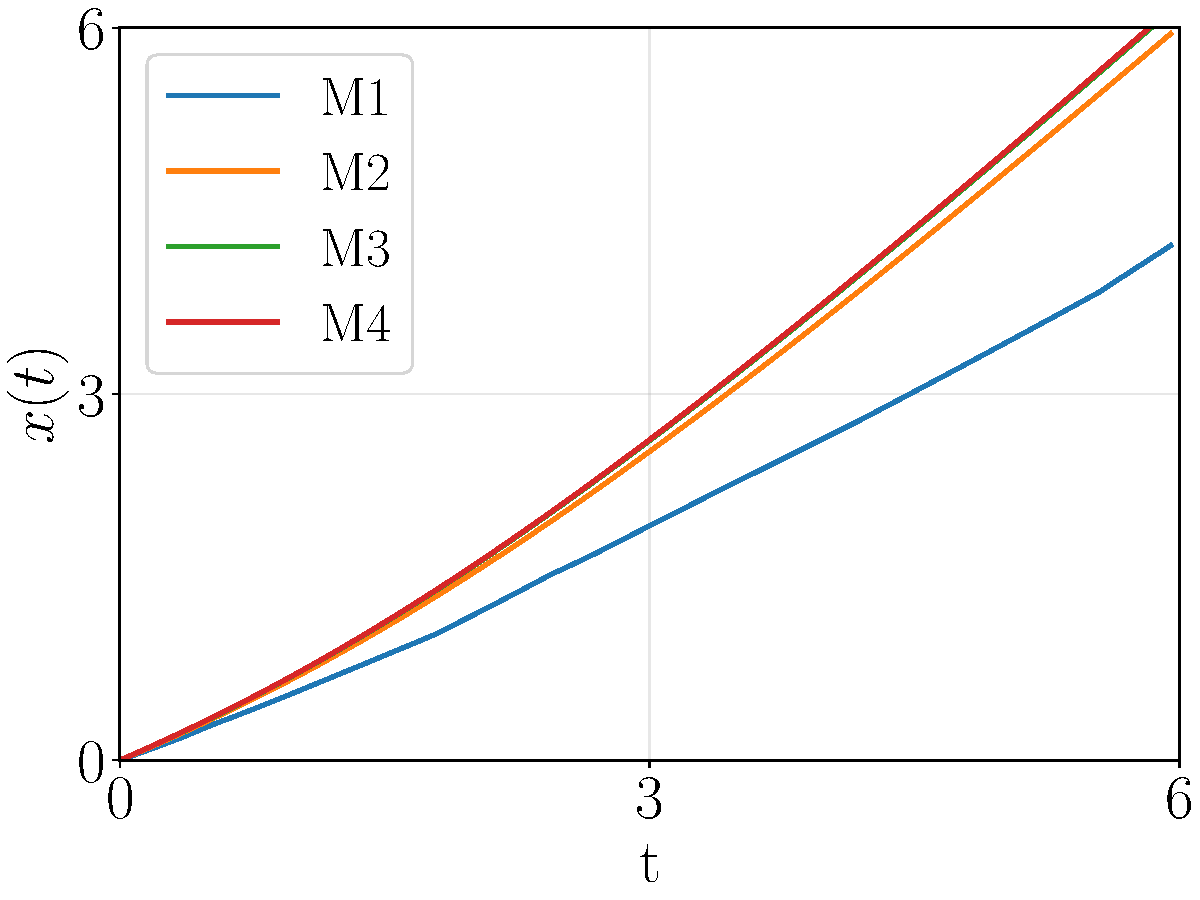
\includegraphics[width=\linewidth]{mesh_conv/stokes_mesh_conv.pdf}
    \caption{Mesh convergence.}
  \end{subfigure}\hspace{0.4cm}
  \begin{subfigure}[b]{0.31\linewidth}
    \centering
    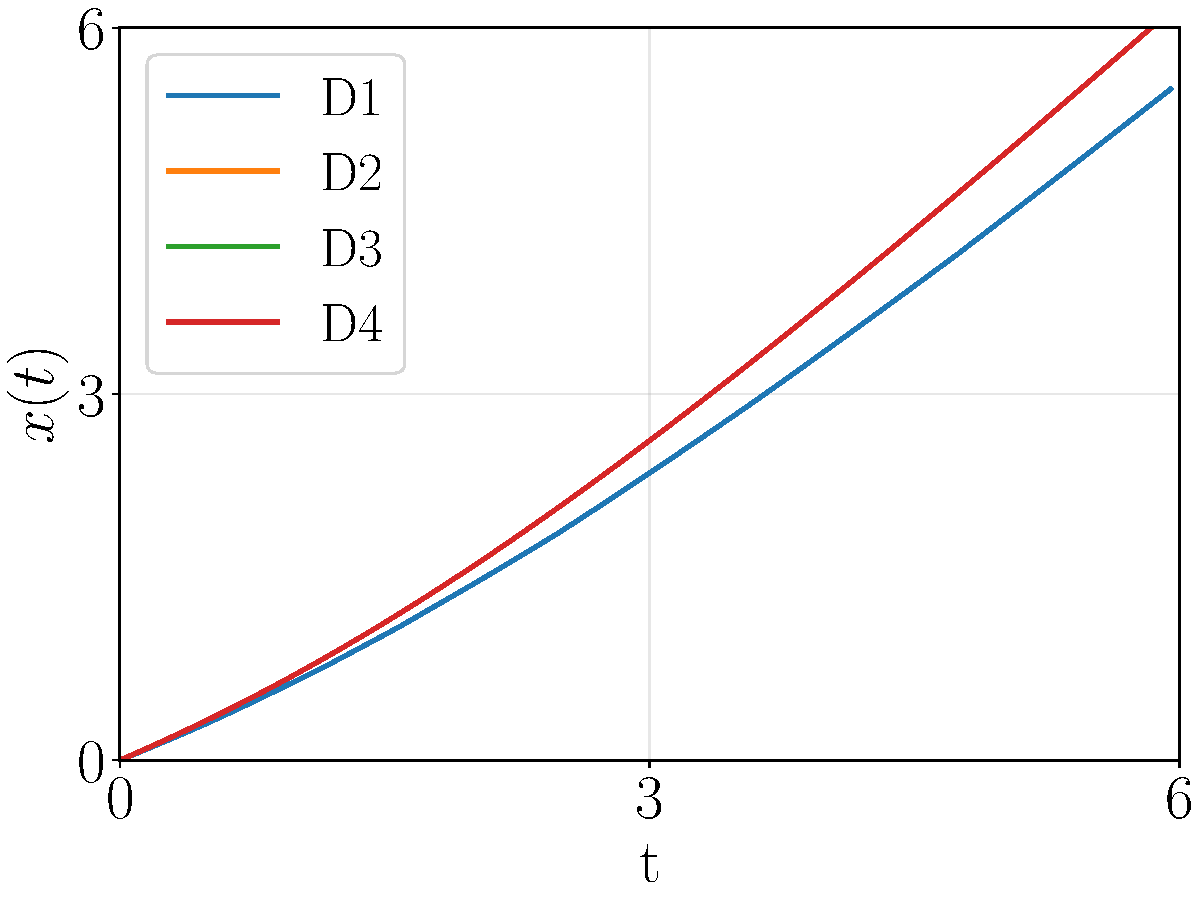
\includegraphics[width=\linewidth]{mesh_conv/stokes_domain_conv.pdf}
    \caption{Domain-size convergence.}
  \end{subfigure}
  \caption{3D bounded geometry ($\delta/a = 0.1$): (a) effect of mesh
           refinement on domain D2 and (b) effect of domain size for
           the converged mesh (Newtonian fluid).}
  \label{fig:stokes_conv_3d}
\end{figure}

\begin{figure}[!ht]
  \centering
  \begin{subfigure}[b]{0.33\linewidth}
    \centering
    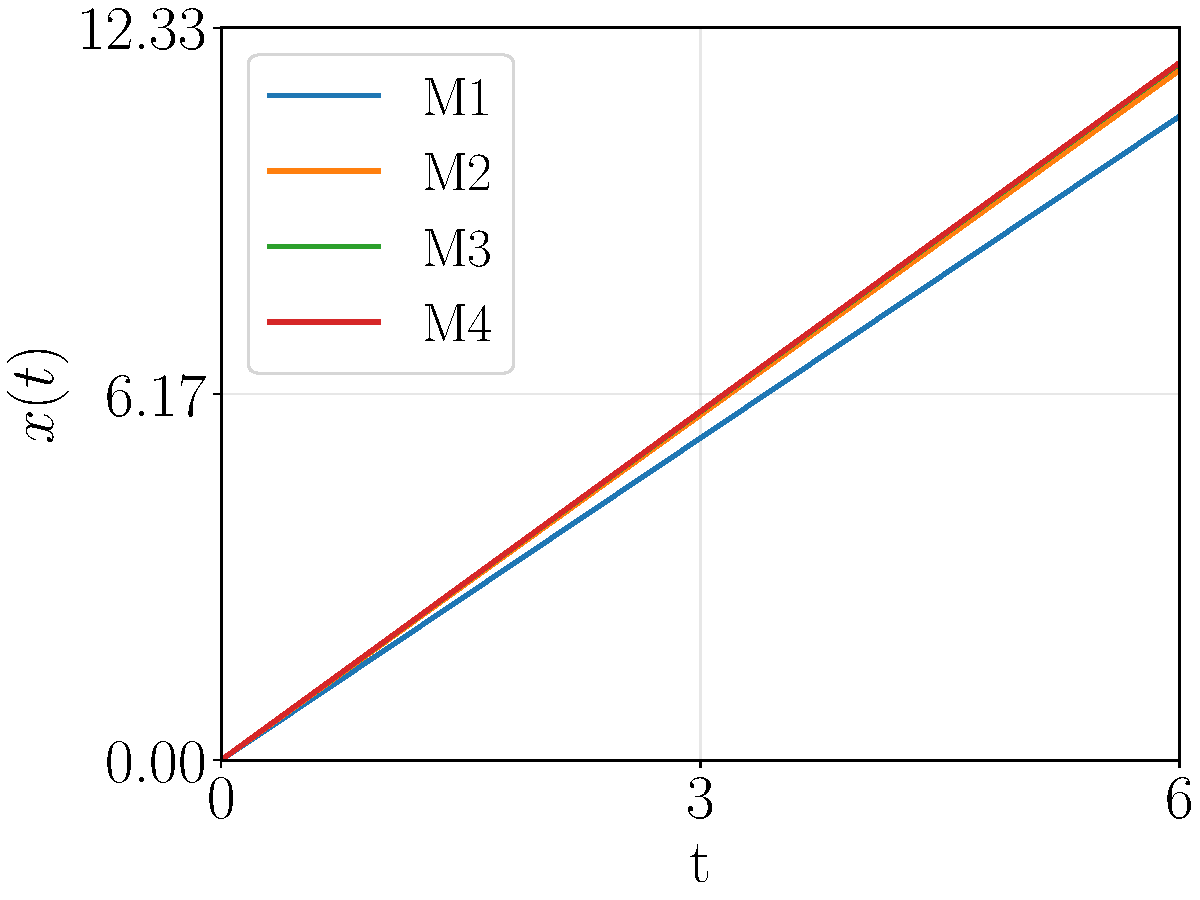
\includegraphics[width=\linewidth]{mesh_conv/stokes_axi_mesh.pdf}
    \caption{Mesh convergence.}
  \end{subfigure}\hspace{0.4cm}
  \begin{subfigure}[b]{0.33\linewidth}
    \centering
    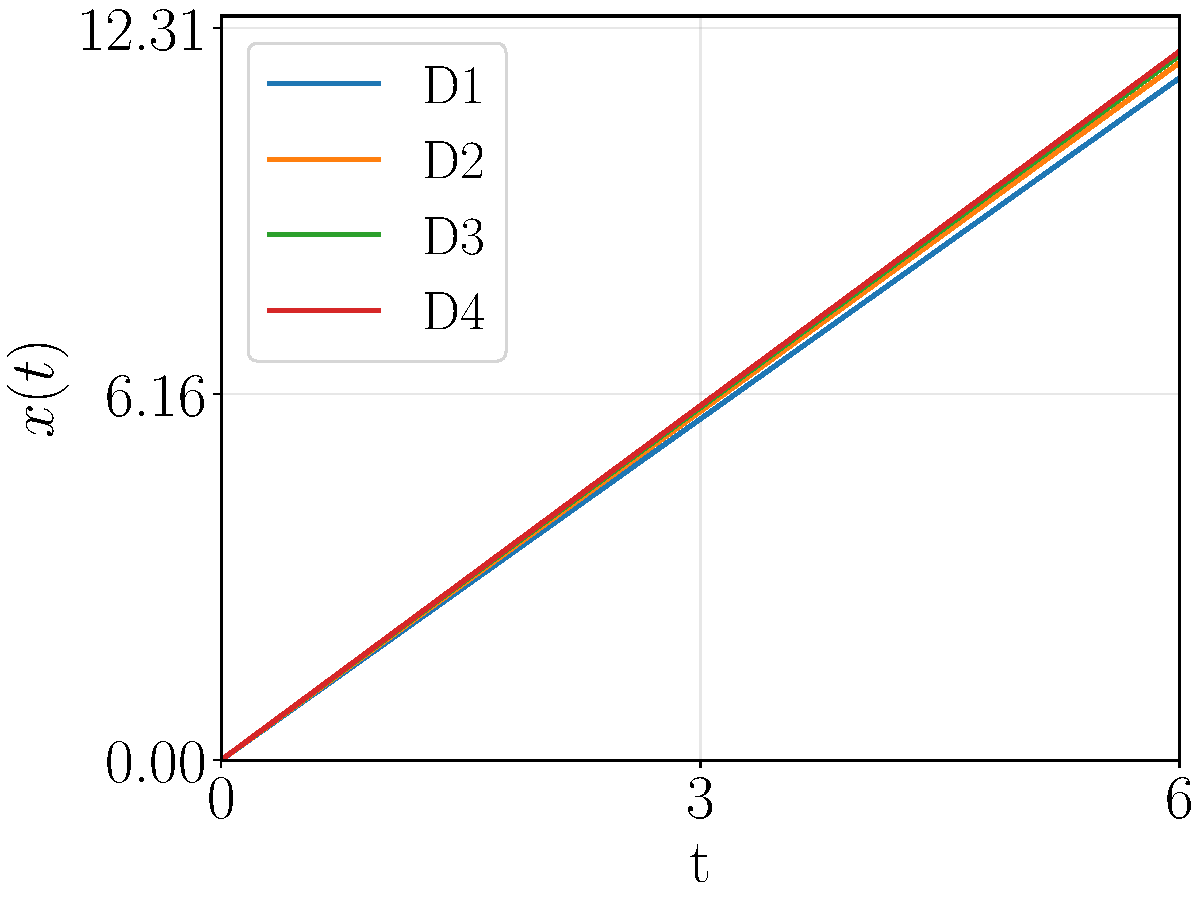
\includegraphics[width=\linewidth]{mesh_conv/stokes_axi_domain.pdf}
    \caption{Domain-size convergence.}
  \end{subfigure}
  \caption{Axisymmetric unbounded geometry: (a) effect of mesh
           refinement on domain D2 and (b) effect of domain size for
           the converged mesh (Newtonian fluid).}
  \label{fig:stokes_conv_axi}
\end{figure}

\FloatBarrier

\subsection{Viscoelastic}

\begin{figure}[!ht]
  \centering
  \begin{subfigure}[b]{0.33\linewidth}
    \centering
    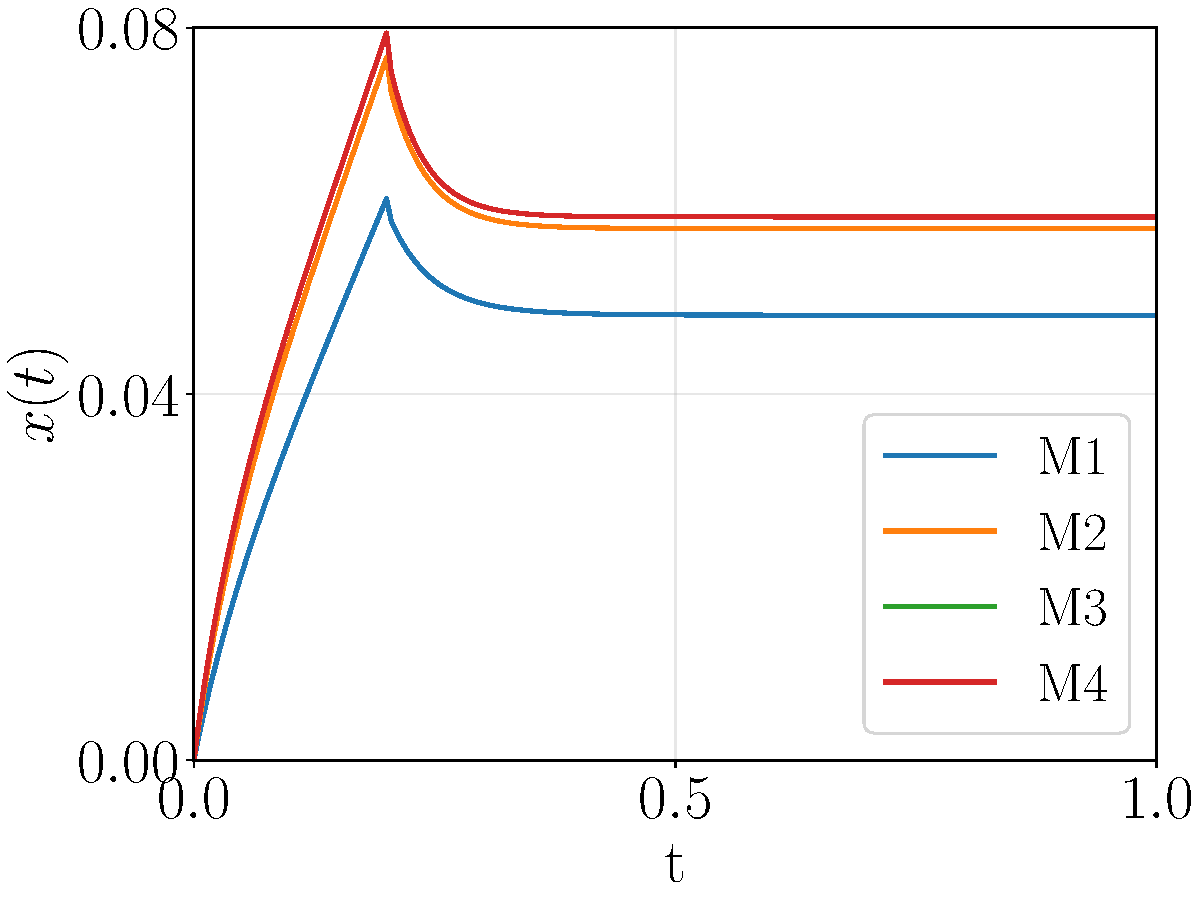
\includegraphics[width=\linewidth]{mesh_conv/creep_mesh_conv.pdf}
    \caption{Mesh convergence.}
  \end{subfigure}\hspace{0.4cm}
  \begin{subfigure}[b]{0.33\linewidth}
    \centering
    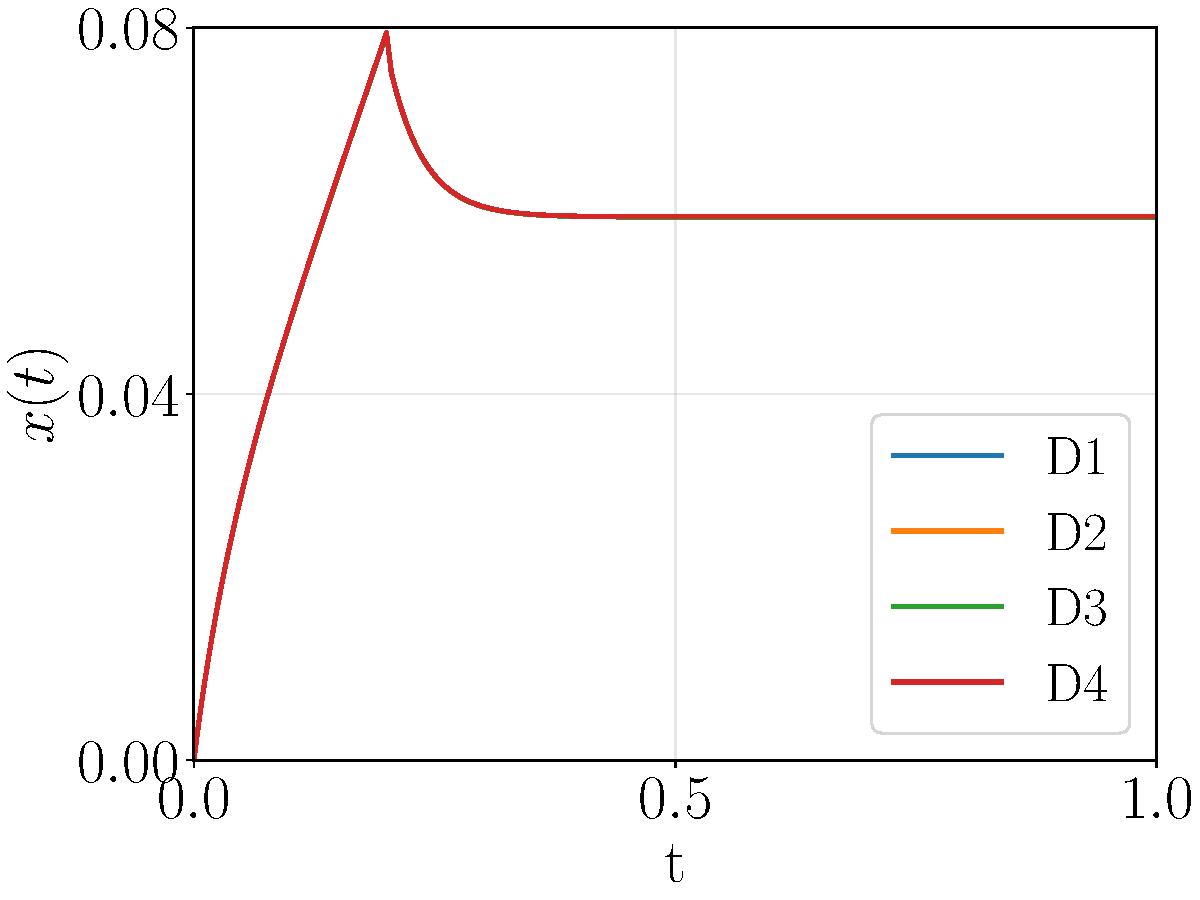
\includegraphics[width=\linewidth]{mesh_conv/creep_domain_conv.pdf}
    \caption{Domain-size convergence.}
  \end{subfigure}
  \caption{3D bounded geometry ($\delta/a = 0.1$): (a) effect of mesh
           refinement on domain D2 and (b) effect of domain size for
           the converged mesh (viscoelastic fluid).}
  \label{fig:creep_3d}
\end{figure}

\begin{figure}[!ht]
  \centering
  \begin{subfigure}[b]{0.33\linewidth}
    \centering
    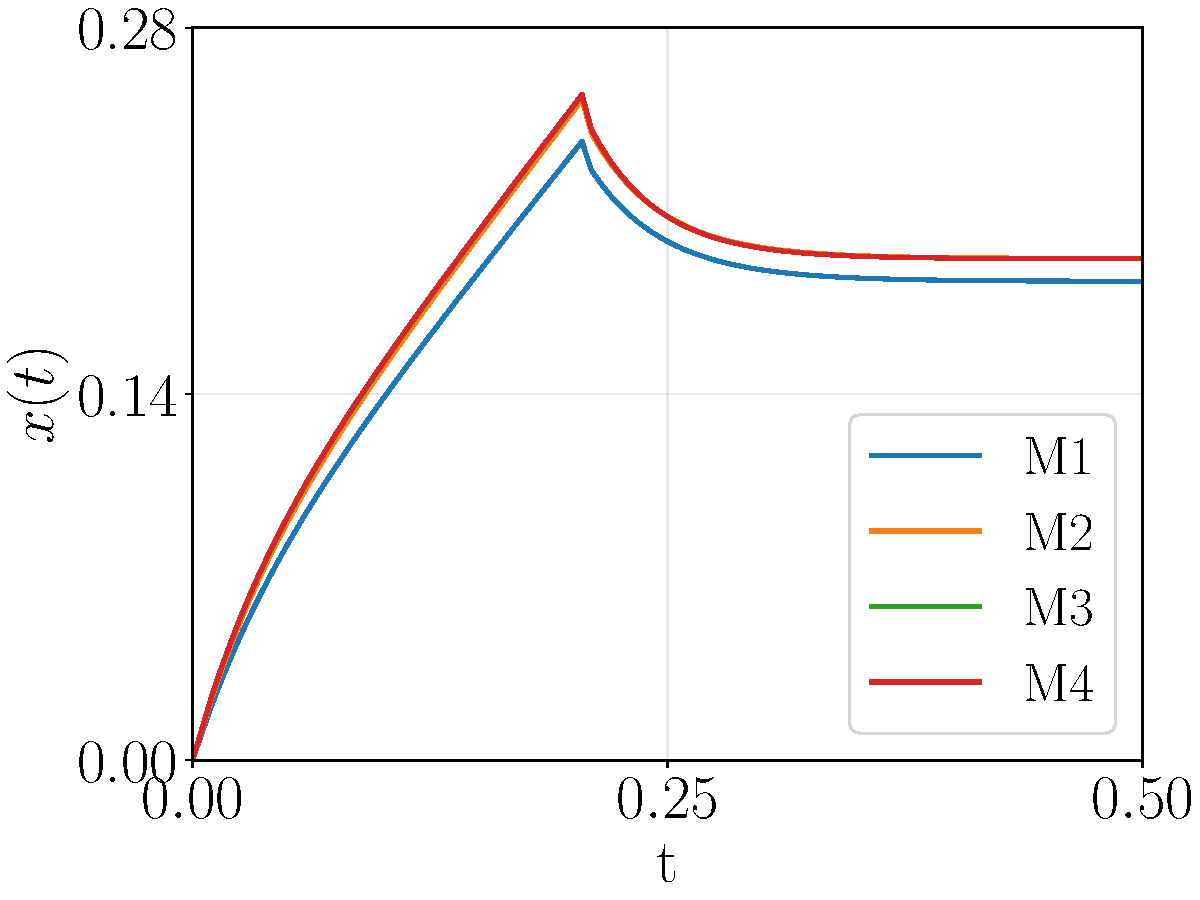
\includegraphics[width=\linewidth]{mesh_conv/creep_axi_mesh.pdf}
    \caption{Mesh convergence.}
  \end{subfigure}\hspace{0.4cm}
  \begin{subfigure}[b]{0.33\linewidth}
    \centering
    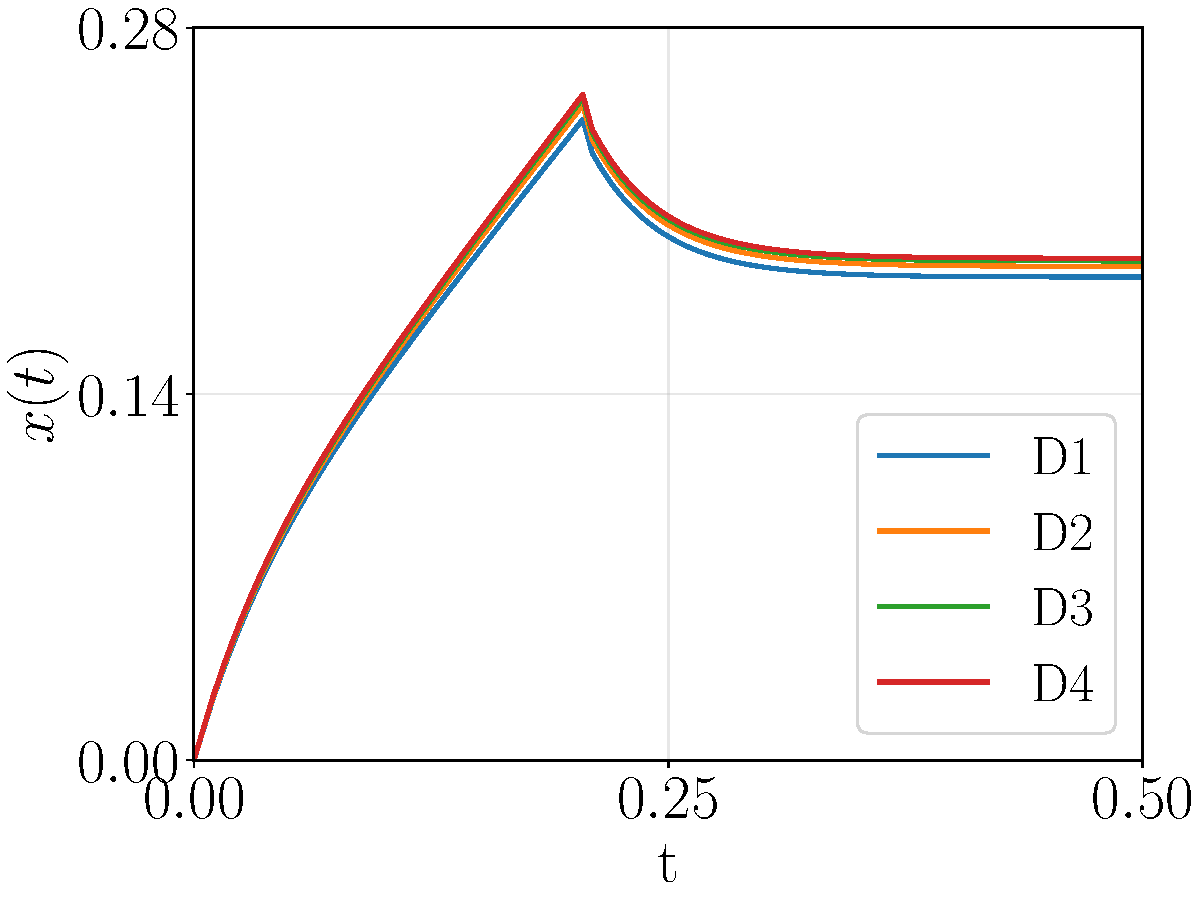
\includegraphics[width=\linewidth]{mesh_conv/creep_axi_domain.pdf}
    \caption{Domain-size convergence.}
  \end{subfigure}
  \caption{Axisymmetric unbounded geometry: (a) effect of mesh
           refinement on domain D2 and (b) effect of domain size for
           the converged mesh (viscoelastic fluid).}
  \label{fig:creep_axi}
\end{figure}

\FloatBarrier

\section{Modeling the heterogeneous microstructure}
\label{sec:blobs}

The models so far assume a spatially homogeneous fluid. To probe a
material whose elasticity varies in space (Section~\ref{sec:heterogeneous_inference}),
we now equip the full-order model with a transported microstructure whose
parameters we likewise aim to infer.
We introduce a scalar concentration field $\phi(\vec{x},t)$ that
modulates the local elasticity of the fluid. It is initialized as a
collection of spherical blobs seeded at randomly placed centers
$\vec{x}_{k}$, each contributing a non-truncated Gaussian profile,
\begin{equation}
\phi_{k}(\vec{x}) = \phi_{\mathrm{blob}}\,
\exp\!\left(-\frac{r_{k}^{2}}{2\,w^{2}}\right),
\qquad r_{k} = \|\vec{x}-\vec{x}_{k}\|,
\label{eq:blob_profile}
\end{equation}
where $\phi_{\mathrm{blob}}$ is the peak concentration and $w$ is its
width. The centers are placed at random and may overlap; their number is
fixed by a prescribed nominal volume fraction.

The field is then transported by the flow, satisfying the following advection equation
\begin{equation}
\frac{\partial \phi}{\partial t} + \vec{u}\cdot\nabla\phi = 0
\quad \text{in } \Omega \setminus P,
\label{eq:phi_advect}
\end{equation}
discretized with the same second-order semi-implicit scheme as the flow
problem. The concentration enters the constitutive model through the local modulus,
while the relaxation time is kept fixed:
\begin{equation}
G(\phi) = \frac{\eta_{\mathrm{p}}}{\lambda}\,\phi,
\qquad \lambda(\phi)\equiv\lambda,
\label{eq:G_of_phi}
\end{equation}
so that the microstructure changes only through the modulus. Since the polymeric
stress is $\ten{\tau}_{\mathrm{p}} = G(\phi)\,(\ten{c}-\ten{I})$, the
varying $G(\phi)$ is evaluated point-wise at every Gauss point from the
convected field, giving a fluid whose local elasticity tracks the
transported microstructure and a particle that experiences a
heterogeneous, evolving viscoelastic environment.

\bibliographystyle{elsarticle-num}
\bibliography{references}

\end{document}
